\documentclass[cs4size,a4paper]{ctexart}   
%==================== 数学符号公式 ============
\usepackage{amsmath}                 % AMS LaTeX宏包
\usepackage[style=1]{mdframed}
\usepackage{amsthm}
\usepackage{amsfonts}
\usepackage{amssymb}
\usepackage{yhmath}
\usepackage{mathrsfs}                % 英文花体字 体
\usepackage{bm}                      % 数学公式中的黑斜体
\usepackage{bbding,manfnt}           % 一些图标,如 \dbend
\usepackage{lettrine}                % 首字下沉,命令\lettrine
\def\attention{\lettrine[lines=2,lraise=0,nindent=0em]{\large\textdbend\hspace{1mm}}{}}
\usepackage{longtable}
\usepackage[toc,page]{appendix}
\usepackage{geometry}                % 页边距调整
\geometry{top=3.0cm,bottom=2.7cm,left=2.5cm,right=2.5cm}
%====================公式按章编号==========================
\numberwithin{equation}{section}
\numberwithin{table}{section}
\numberwithin{figure}{section}
%================= 基本格式预置 ===========================
\usepackage{fancyhdr}
\pagestyle{fancy}
\fancyhf{}  
\fancyhead[C]{\zihao{5}  \kaishu 概率的悖论——公理化的意义}
\fancyfoot[C]{~\zihao{5} \thepage~}
\renewcommand{\headrulewidth}{0.65pt} 
\CTEXsetup[format={\centering\bfseries\zihao{-2}},name={第, 章}]{section}
\CTEXsetup[nameformat={\bfseries\zihao{3}}]{subsection}
\CTEXsetup[nameformat={\bfseries\zihao{4}}]{subsubsection}
%================== 图形支持宏包 =========================
\usepackage{subfigure}
\usepackage{graphicx}                % 嵌入png图像
\usepackage{color,xcolor}            % 支持彩色文本、底色、文本框等
\usepackage{hyperref}                % 交叉引用
\usepackage{caption}
\captionsetup{figurewithin=section}
%==================== 源码和流程图 =====================
\usepackage{listings}                % 粘贴源代码
\usepackage{xcolor}
\usepackage{color}
\definecolor{dkgreen}{rgb}{0,0.6,0}
\definecolor{gray}{rgb}{0.5,0.5,0.5}
\definecolor{mauve}{rgb}{0.58,0,0.82}
 \usepackage{xcolor}
 \lstset{
  %行号
    numbers=left,
    %背景框
    framexleftmargin=8mm,
    frame=none,
     %背景色
    %backgroundcolor=\color[rgb]{1,1,0.76},
     backgroundcolor=\color[RGB]{245,245,244},
     %样式
   keywordstyle=\bf\color{blue},
   identifierstyle=\bf,
    numberstyle=\color[RGB]{0,192,192},
    commentstyle=\it\color[RGB]{0,96,96},
   stringstyle=\rmfamily\slshape\color[RGB]{128,0,0},
   %显示空格
    showstringspaces=false
 }


%--------------------
\hypersetup{hidelinks}
\usepackage{booktabs}  
\usepackage{shorttoc}
\usepackage{tabu,tikz}
\usepackage{float}

\usepackage{multirow}



\tabcolsep=1ex
\tabulinesep=\tabcolsep
\newlength\tikzboxwidth
\newlength\tikzboxheight
\newcommand\tikzbox[1]{%
        \settowidth\tikzboxwidth{#1}%
        \settoheight\tikzboxheight{#1}%
        \begin{tikzpicture}
        \path[use as bounding box]
                (-0.5\tikzboxwidth,-0.5\tikzboxheight)rectangle
                (0.5\tikzboxwidth,0.5\tikzboxheight);
        \node[inner sep=\tabcolsep+0.5\arrayrulewidth,line width=0.5mm,draw=black]
                at(0,0){#1};
        \end{tikzpicture}%
        }

\makeatletter
\def\hlinew#1{%
  \noalign{\ifnum0=`}\fi\hrule \@height #1 \futurelet
   \reserved@a\@xhline}
   
\newcommand{\tabincell}[2]{\begin{tabular}{@{}#1@{}}#2\end{tabular}}%

\usepackage{subfigure}

\usepackage{CJK}
\usepackage{ifthen}


\usepackage{graphicx} 
\newcommand{\HRule}{\rule{\linewidth}{0.5mm}}

\newtheorem{Theorem}{定理}
\newtheorem{Lemma}{引理} 
%%使得公式随章节自动编号
\makeatletter
\@addtoreset{equation}{section}
\makeatother
\renewcommand{\theequation}{\arabic{section}.\arabic{equation}}

%-------------------------
	
\usepackage{pythonhighlight}
\usepackage{tikz}                    
\usepackage{tikz-3dplot}
\usetikzlibrary{shapes,arrows,positioning}
%===================   正文开始    ===================
\begin{document}
\bibliographystyle{gbt7714-2005}     %论文引用格式
%===================  定理类环境定义 ===================
\newtheorem{example}{例}              % 整体编号
\newtheorem{algorithm}{算法}
\newtheorem{theorem}{定理}            % 按 section 编号
\newtheorem{definition}{定义}
\newtheorem{axiom}{公理}
\newtheorem{property}{性质}
\newtheorem{proposition}{命题}
\newtheorem{lemma}{引理}
\newtheorem{corollary}{推论}
\newtheorem{remark}{注解}
\newtheorem{condition}{条件}
\newtheorem{conclusion}{结论}
\newtheorem{assumption}{假设}
%==================重定义 ===================
\renewcommand{\contentsname}{目录}
\renewcommand{\abstractname}{摘要}
\renewcommand{\refname}{参考文献}
\renewcommand{\indexname}{索引}
\renewcommand{\figurename}{图}
\renewcommand{\tablename}{表}
\renewcommand{\appendixname}{附录}
\renewcommand{\proofname}{证明}
\renewcommand{\algorithm}{算法}
%============== 封皮和前言 =================

\maketitle

\section*{数据链路层实验}
\pagestyle{plain}
\pagenumbering{Roman}
\section*{\zihao{2} \centering 摘要}

\vskip0.5cm
和所有的数学分支类似,概率论的也是经历了从直觉到严格的过程,其中的一个转
折点就是贝特朗悖论.在概率论的发展史上, 贝特朗悖论起了揭示问题促使人们思考概率
理论体系严密性的作用. 最后, 前苏联数学家柯尔莫哥洛夫建立了概率论的公理化体
系. 在概率论的公理化以及数学的发展, 悖论起到了重要的作用.


\textbf{关键词:}  贝特朗悖论,几何概率, 样本空间, 等可能假设, 概率的公理化
\addcontentsline{toc}{section}{摘要}

\section*{\zihao{2} \centering 介绍}

本主要对悖论及贝特朗悖论做出了阐释, 并列出其3种不同的解法. 其内涵是对“等可能”这一论述的不同解释, 从而引出概率公理化的必要性.

\addcontentsline{toc}{section}{介绍}
\pagestyle{empty}
\tableofcontents
\thispagestyle{empty}
%============== 论文正文   =================
\pagestyle{fancy}
\pagenumbering{arabic}

\section{概率的悖论}

\subsection{悖论}

悖论是一逻辑学术语,指那些会导致逻辑矛盾的命题.如果承认这个命题成立,就
可推出它的否定命题成立;反之,如果承认这个命题的否定命题成立,又可推出这个命题
成立.像这样自相矛盾的命题就是悖论.
\par 悖论是表面上同一命题或推理中隐含着两个对立的结论,而这两个结论都能自圆其
说.悖论的抽象公式就是:如果事件A发生,则推导出非A,非A发生则推导出A.
\par 古今中外有不少著名的悖论,它们震撼了逻辑和数学的基础,激发了人们求知和精
密的思考,吸引了古往今来许多思想家和爱好者的注意力.解决悖论难题需要创造性的
思考,悖论的解决又往往可以给人带来全新的观念.

\subsection{贝特朗悖论}
“在一个圆内任意选一条弦,这条弦的弦长长于这个圆的内接等边三角形的边长的
概率是多少?”

\subsubsection{问题提出}
几何概率是十九世纪末新发展起来的一门学科,使很多概率问题的解决变得简单而
不用运用微积分的知识.而正当几何概型正如火如荼的发展时,法国学者贝特朗于1899
年针对几何概念提出了这样一个“简单”的问题,并在当时数学界引起了轩然大波.按照几何概率的定义进行计算,
竟然可以求得3个不同的概率,这与概率的性质是背道而驰的.这就是后来人们熟知的贝特朗悖
论,矛头直指几何概率概念本身.

\subsubsection{三种解法}
首先,关于几何概型和几何概率,有如下定义,若随机试验$E$具有以下特点:
\par (1) 样本空间是直线或二维、三维空间中的度量有限的区间或区域;
\par (2) 样本点在其上是均匀分布的(即所有基本事件是等可能的).\\
则这样的随机试验称为几何概型.在几何概型中,若样本空间$\Omega$所对应区域的度量
为$L(\Omega)$,且事件$A$的度量为$L(A)$,则事件$A$的概率为
\[
	P(A) = \dfrac{L(A)}{L(\Omega)}.
\]
在贝特朗问题提出时,贝特朗就提出了3种经典的解法:

\paragraph*{方法一} 任意弦交圆周于两点,不妨将弦的一段$A$固定,问题化为在圆周上任取另一端
点$B$.这时,样本空间$\Omega$为圆周上任一点,假设任一点的选取具有等可能性.如图1.1(a)
所示,以$A$为顶点做一等边三角形$AMN$,显然弦$AB$的长度大于$\sqrt{3}$当且仅当端点$B$
落在$\wideparen{MN}$上.而$\wideparen{MN}$的长为整个圆周的$\dfrac{1}{3}$,于是所求概率为$\dfrac{1}{3}$.

\paragraph*{方法二} 如图1.1(b)所示,不妨只考虑与直径$MN$垂直的弦,样本空间$\Omega$为$MN$上任
一点,假设弦$AB$的中点在$MN$上是等可能的.当且仅当弦$AB$与圆心的距离小于$\dfrac{1}{2}$
时,弦$AB$的长度大于$\sqrt{3}$,于是所求概率为$\dfrac{1}{2}$.

\paragraph*{方法三} 如图1.1(c)所示,弦被其中点唯一确定,假设弦的中点在圆周内是等可能的.当
且仅当弦$AB$的中点在半径为$\dfrac{1}{2}$的同心圆内时,弦$AB$的长度大于$\sqrt{3}$,此小圆面积为
大圆面积的$\dfrac{1}{4}$,于是所求概率为$\dfrac{1}{4}$.

\begin{figure}[thbp!]
	\centering
	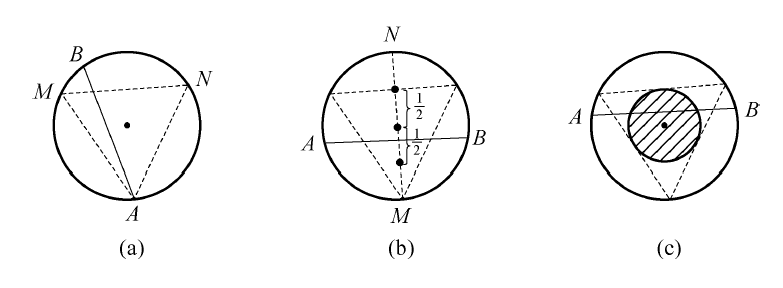
\includegraphics[width=0.8\linewidth]{figure/circ.png}
	\caption{}
	\label{fig:circ}
\end{figure}

由于在取弦时采用了3种不同的等可能假设,对3种不同的随机试验得到了3种不
同结果,通过分析这3种结果均正确.而这这严重违背了常理.

\subsubsection{观点争执}
贝特朗问题之所以出现3种不同的答案,是因为人们观察随机试验的基本结果的角
度不同,同时对基本结果的等可能性假设也有不同的理解.

\par 然而,仍然有不少学者对此持怀疑态度,并根据自己对问题的理解以及自己特有的
思维方式,钟情于其中的某种解法,想方设法寻找其他解法的瑕疵,推翻其他解法的合理
性,从而认为贝特朗悖论并不奇,答案其实是唯一的.      %
\section{预备知识}

本章是正式开始研究两个大问题之前的准备工作, 主要介绍了欧氏空间、线性变
换、向量范数、矩阵范数以及矩阵函数, 这些都是之后研究问题的基石.

\subsection{欧式空间与线性变换}

本节研究欧氏空间及线性变换的性质, 特别是几种重要的线性变换、对若尔当标准形的求解和线性变换的求法.

\subsubsection{欧式空间与线性变换介绍}

\paragraph*{线性空间} \

\par 线性空间是线性代数中最基本的概念之一, 也是学习现代矩阵论的重要基础. 线性空间的概念, 是某类事物从量的方面的一个抽象. 我们不考虑集合的对象, 抽去它们的具体内容的含义, 来研究这类集合的公共性质, 并引进一个概括性名词. 于是就有如下的线性空间的概念.

\paragraph*{定义 2.1} 设 $V$ 是一个非空集合, 他的元素用 $\bm{x},\bm{y},\bm{z}$ 等表示, 并称之为向量; $K$ 是一个数域, 它的元素用 $k, l, m$ 等表示. 如果 $V$ 满足条件:
\par (1) 在$V$中定义一个加法运算, 即当 $\bm{x}, \bm{y} \in V$ 时, 有唯一的和 $\bm{x} + \bm{y} \in V$, 且加法运算满足以下性质:
\par 1) 结合律 $\bm{x} + (\bm{y} + \bm{x}) = (\bm{x} + \bm{y}) = \bm{z}$;
\par 2) 交换律 $\bm{x} + \bm{y} = \bm{y} + \bm{x}$;
\par 3) 存在零元素 $\bm{0}$, 使 $\bm{x} + \bm{0} = \bm{x}$;
\par 4) 存在负元素, 即对任一向量 $\bm{x}\in V$, 存在向量 $\bm{y} \in V$, 使 $\bm{x + y = 0}$, 则称$\bm{y}$ 为 $\bm{x}$
的负元素, 记为$\bm{-x}$, 于是有 $\bm{x + (- x) = 0}$.
\par (2) 在 $V$ 中定义数乘(数与向量的乘法)运算, 即当 $\bm{x} \in V, k \in K$ 时, 有唯一的乘
积 $k\bm{x} \in V$, 且数乘运算满足以下性质:
\par 5) 数因子分配律 $k(\bm{x + y} = k \bm{x} + k \bm{y})$;
\par 6) 分配律 $(k + l) \bm{x} = k \bm{x} + l \bm{x}$;
\par 7) 结合律 $k(l \bm{x}) = (kl) \bm{x}$;
\par 8) $1 \cdot \bm{x} = \bm{x}$ \\
则称 $V$ 为数域 $K$ 上的线性空间或向量空间.

\par $V$中所定义的加法及数乘运算统称为 $V$ 的线性运算. 在不致产生混淆时, 将数域 $K$ 上的
线性空间简称为线性空间. 数 $k$ 与向量 $\bm{x}$ 的乘积$k\bm{x}$也可写成$\bm{x}k$.

\par 需要指出, 不管$V$的元素如何, 当$K$为实数域$\mathbb{R}$时, 则称$V$为实线性空间; 当$K$为复
数域$\mathbb{C}$时, 就称$V$为复线性空间.

\paragraph*{例 2.1} 设$\mathbb{R^{+}}$为所有正实数组成的数集, 其加法与数乘运算分别定义为
$$
    m \oplus n = mn, \quad k \circ m = m^k
$$
证明$\mathbb{R^{+}}$是$\mathbb{R}$是上的线性空间. \par

\paragraph*{证} 设$m,n\in \mathbb{R^+}, \quad k \in R$,则有
$$
    m \oplus n = mn \in \mathbb{R^+}, \quad k \circ m = m^k \in \mathbb{R^+}
$$
即$\mathbb{R^+}$对所定义的加法运算“$\oplus$”与数乘运算“$\circ$”是封闭的,且有

\par (1) $(m \oplus n) \oplus p = (mn) \oplus p = mnp = m \oplus (np) = m \oplus (n \oplus p)$
\par (2) $m \oplus n = mn = nm = n \oplus m$
\par (3) 1是零元素,因为$m \oplus 1 = m \times 1 = m$
\par (4) $m$的负元素是$\dfrac{1}{m}$,因为$m \oplus \dfrac{1}{m} = m \oplus \dfrac{1}{m} = 1$
\par (5) $k \circ (m \oplus n) = k \circ (mn) = (mn)^k = m^kn^k = (k \circ m) \oplus (k \circ n)$
\par (6) $(k + l) \circ m = m^{k + l} = m^km^l = (k \circ m) \oplus (l \circ m)$
\par (7) $k \circ (l \circ m) = k \circ m^l = m^{lk} = m^{kl} = (kl) \circ m$
\par (8) $1 \circ m = m^1 = m$
\\ 成立, 故$\mathbb{R^+}$是实线性空间.

\paragraph*{定义 2.2} 设 $V$ 是数域 $K$ 上的线性空间, $\bm{x}_1,\bm{x}_2,\cdots,\bm{x}_r(r\geqslant 1)$ 是属于 $V$ 的任意 $r$ 个
向量, 如果它满足
\par (1) $\bm{x}_1,\bm{x}_2,\cdots,\bm{x}_r$ 线性无关;
\par (2) $V$ 中任一向量 $x$ 都是 $\bm{x}_1,\bm{x}_2,\cdots,\bm{x}_r$ 的线性组合.
\\ 则称 $\bm{x}_1,\bm{x}_2,\cdots,\bm{x}_r$ 为 $V$ 的一个基或基底, 并称 $\bm{x}_i(i=1,2,\cdots,r)$ 为基向量.

\par 且由上述定义可见, 线性空间的维数是其基中所含向量的个数.

\par 同时, 一个线性空间的基不是唯一的. 例如, $n$ 维向量组
\begin{gather}
    \begin{cases}
        \bm{e}_1 = (1, 0, \cdots, 0) \\
        \bm{e}_2 = (0, 1, \cdots, 0) \\
        \cdots                       \\
        \bm{e}_n = (0, 0, \cdots, 1)
    \end{cases}
    \begin{cases}
        \bm{y}_1 = (1, 1, \cdots, 1, 1) \\
        \bm{y}_2 = (0, 1, \cdots, 1, 1) \\
        \cdots                          \\
        \bm{y}_n = (0, 0, \cdots, 0, 1)
    \end{cases}
    \tag{2.1.1} \label{2.1.1}
\end{gather}
都实线性空间 $\bm{R}^n$ 的基. 这是因为
$$
    \begin{vmatrix}
        1      & 0      & \cdots & 0      \\
        0      & 1      & \cdots & 0      \\
        \vdots & \vdots &        & \vdots \\
        0      & 0      & \cdots & 1
    \end{vmatrix} \neq 0, \quad
    \begin{vmatrix}
        1      & 1      & \cdots & 1      & 1      \\
        0      & 1      & \cdots & 1      & 1      \\
        \vdots & \vdots &        & \cdots & \vdots \\
        0      & 0      & \cdots & 0      & 1
    \end{vmatrix} \neq 0, \quad
$$
从而它们各自都线性无关, 而且对于任一向量 $\bm{x} = (\xi_1, \xi_2, \cdots, \xi_n) \in R^n$, 分别有
\begin{gather*}
    \bm{x} = \xi_1\bm{e}_1 + \xi_2\bm{e}_2 + \cdots + \xi_n\bm{e}_n \\
    \bm{x} = \xi_1\bm{y}_1 + (\xi_2 - \xi_1)\bm{y}_2 + \cdots + (\xi_n - \xi_{n - 1})\bm{y}_n
\end{gather*}

\paragraph*{定义 2.3} 称线性空间 $V^n$ 的一个基 $\bm{x}_1,\bm{x}_2,\cdots,\bm{x}_r$ 为 $V^n$ 的一个坐标系. 设向量 $\bm{x} \in V^n$, 它在该基下的线性表示式为
$$
    \bm{x} = \xi_1 \bm{x}_1 + \xi_2 \bm{x}_2 + \cdots + \xi_n \bm{x}_n
$$
则称$\xi_1, \xi_2, \cdots, \xi_n$ 为 $\bm{x}$ 在该坐标系中的坐标或分量, 记为
$$
    (\xi_1, \xi_2, \cdots, \xi_n)^T
$$

\par 需要指出, 在不同的坐标系(或基)中, 同一向量的坐标一般是不同的.

\paragraph*{欧氏空间} \

\par 欧式空间是一种特殊的线性空间, 定义如下.

\paragraph*{定义 2.4} 设 $V$ 是实数域 $\mathbb{R}$ 上的线性空间, 对于 $V$ 中任意两个向量 $\bm{x}$ 与 $\bm{y}$, 按照某种规则定义一个实数, 用 $(\bm{x}, \bm{y})$ 来表示, 且它满足下述4个条件:
\par (1) 交换律: $(\bm{x}, \bm{y}) = (\bm{y}, \bm{x})$;
\par (2) 分配律: $(\bm{x}, \bm{y} + \bm{z}) = (\bm{x}, \bm{y}) + (\bm{x}, \bm{z})$;
\par (3) 齐次性: $(k\bm{x}, \bm{y}) = k(\bm{x}, \bm{y})(\forall k \in \mathbb{R})$;
\par (4) 非负性: $(\bm{x}, \bm{x}) \geqslant 0$, 当且仅当 $\bm{x} = \bm{0}$ 时, $(\bm{x}, \bm{x}) = 0$.
\\ 则称实数 $(\bm{x}, \bm{y})$ 为向量 $\bm{x}$ 与 $\bm{y}$ 的内积, 而称 $V$ 为Euclid空间, 简称欧氏空间或实内积空间.

\par 显然, 欧氏空间是定义了内积的实线性空间. 因此, 又有内积空间之称, 可见, 欧氏空间是一个特殊的实线性空间.

\par 因为向量的内积与向量的线性运算是彼此无关的运算, 所以不论内积如何规定, 都
不会影响该实线性空间的维数. 欧氏空间的子空间显然也是欧氏空间.

\paragraph[]{线性变换} \

\par 线性空间是某类客观事物从量的方面的一个抽象, 而线性变换则研究线性空间中元素之间的最基本联系.

\paragraph*{定义 2.5} 设 $V$ 是数域 $K$ 上的线性空间, $T$ 是 $V$ 到自身的一个映射, 使对任意向量
$\bm{x} \in V$, $V$ 中都有唯一的向量 $\bm{y}$ 与之对应, 则称 $T$ 是 $V$ 的一个变换或算子, 记为 $T\bm{x} = \bm{y}$,
称 $\bm{y}$ 为 $\bm{x}$ 在 $T$ 下的象, 而 $\bm{x}$ 是 $\bm{y}$ 的原象(或象源).

\par 例如, 平面上所有起点在原点的向量的集合, 形成实二维线性空间 $R^2$. 在 $R^2$ 中绕
原点的旋转就是 $R^2$ 的一个变换.

\paragraph*{定义 2.6} 如果数域 $K$ 上的线性空间 $V$ 的一个变换 $T$ 具有以下性质:
$$
    T(k\bm{x} + l\bm{y}) = k(T\bm{x}) + l(T\bm{y})
$$
其中 $\bm{x}, \bm{y} \in V, k, l \in K$. 则称 $T$ 为 $V$ 的一个线性变换或线性算子.

\paragraph*{例 2.2} 把线性空间 $R^2$ 的所有向量均绕原点依顺(或逆)时针方向旋转 $\theta$ 角的变换, 就是一个线性变换. 这时象 $(\eta_1, \eta_2)$ 与原象 $(\xi_1, \xi_2)$之间的关系为
$$
    \begin{bmatrix}
        \eta_1 \\
        \eta_2
    \end{bmatrix} = \begin{bmatrix}
        \cos\theta  & \sin\theta \\
        -\sin\theta & \cos\theta
    \end{bmatrix} \begin{bmatrix}
        \xi_1 \\
        \xi_2
    \end{bmatrix}
$$

\paragraph*{例 2.3} 在线性空间 $P_n$ 中, 求微分是其一个线性变换, 这里用 $D$ 表示, 即
$$
    Df(t) = f'(t) \quad (\forall f(t) \in P_n)
$$
\par 事实上, 对任意的 $f(t), g(t) \in P_n$ 及 $k, l \in \mathbb{R}$, 有
$$
    D(kf(t) + lg(t)) = (kf(t) + lg(t))' = kf'(t) + lg'(t) = k(Df(t)) + l(Dg(t))
$$

\par 不过需要注意, 线性变换可能把线性无关的向量组变为线性相关的向量组. 如零变
换 $T_0$ 就是这样.

\paragraph*{定义 2.6} 设 $T$ 是线性空间 $V$ 的线性变换, $V$ 中所有向量的象形成的集合, 称为 $T$ 的
值域, 用 $R(T)$ 表示, 即
$$
    R(T) = \{T\bm{x} \mid \bm{x} \in V \}
$$
$V$ 中所有被 $T$ 变为零向量的原象构成的集合, 称为 $T$ 的核, 用 $N(T)$ 表示, 即
$$
    N(T) = \{\bm{x} \mid T\bm{x} = \bm{0}, \bm{x} \in V \}
$$

\paragraph[]{线性变换的运算} \

\par 下面, 为了讨论线性变换的运算, 引入单位变换的零变换的概念.

\par 把线性空间 $V$ 的任一向量都变为其自身的变换是一个线性变换, 称为单位变换或
恒等变换, 记为 $T_e$, 于是有
$$
    T_e \bm{x} = \bm{0} \quad (\forall \bm{x} \in V)
$$

\par 如果 $T_1, T_2$ 是 $V$ 的两个变换, 且对于任意向量 $\bm{x} \in V$, 都有 $T_1\bm{x} = T_2\bm{x}$, 那么就称
$T_1$ 与 $T_2$ 相等, 记为
$$
    T_1 = T_2
$$

\par 对于线性空间的线性变换, 下面定义它们的集中运算方式.

\par{1.加法}

\par 设 $T_1, T_2$ 是线性空间 $V$ 的两个线性变换, 定义它们的和 $T_1 + T_2$ 为
$$
    (T_1 + T_2) \bm{x} = T_1 \bm{x} + T_2 \bm{x} \quad (\forall \bm{x} \in V)
$$
\par 下面证明, 线性变换 $T_1$ 与 $T_2$ 的和 $T_1 + T_2$ 仍是 $V$ 的线性变换. 事实上, 对任意
$\bm{x}, \bm{y} \in V, k, l \in K$, 由定义2.6有
\begin{align*}
    (T_1 + T_2)(k\bm{x} + l\bm{y}) = & T_1(k\bm{x} + l\bm{y}) + T_2(k\bm{x} + l\bm{y}) =           \\
                                     & k(T_1\bm{x}) + l(T_1\bm{y}) + k(T_2\bm{x}) + l(T_2\bm{y}) = \\
                                     & k(T_1\bm{x} + T_2\bm{x}) + l(T_1\bm{y} + T_2\bm{y}) =       \\
                                     & k(T_1 + T_2)\bm{x} + l(T_1 + T_2)\bm{y}
\end{align*}
这就表明 $T_1 + T_2$ 是 $V$ 的线性变换.

\par 另外, 定义线性变换 $T$ 的负变换 $-T$ 定义为
$$
    (-T)\bm{x} = -(T\bm{x}) \quad (\forall \bm{x} \in V)
$$

\par 因此, 线性变换的加法具有以下基本性质:
\par (1) $T_1 + T_2 = T_2 + T_1$;
\par (2) $(T_1 + T_2) + T_3 = T_1 + (T_2 + T_3)$;
\par (3) $T + T_0 = T$;
\par (4) $T + (-T) = T_0$.

\par{2. 线性变换与数的乘法}

\par 设 $k \in K$, $T$ 为线性空间 $V$ 中的线性变换, 定义数 $k$ 与 $T$ 的乘积 $kT$ 为
$$
    (kT)\bm{x} = k(T\bm{x}) \quad (\forall \bm{x} \in V)
$$

\par 因此, 线性变换的数乘具有以下基本性质:
\par (1) $k(T_1 + T_2) = kT_1 + k$;
\par (2) $(k + l)T = kT + lT$;
\par (3) $(kl)T= k(lT)$;
\par (4) $1\ T = T$.

\par{3. 线性变换的乘法}

\par 设 $T_1, T_2$ 是线性空间 $V$ 的两个线性变换, 定义 $T_1$ 与 $T_2$ 的乘积 $T_1T_2$ 为
$$
    (T_1T_2)\bm{x} = T_1(T_2)\bm{x} \quad (\forall \bm{x} \in V)
$$
即 $T_1T_2$ 是先施行 $T_2$, 然后施行 $T_1$ 的变换. 且
\begin{align*}
    (T_1T_2)(k\bm{x} + l\bm{y}) = & T_1(T_2(k\bm{x} + l\bm{y})) =           \\
                                  & k(T_1(T_2\bm{x})) + l(T_1(T_2\bm{y})) = \\
                                  & k(T_1T_2)\bm{x} + l(T_1T_2)\bm{y}
\end{align*}

\par 因此, 线性变换的乘积具有以下基本性质:
\par (1) $(T_1T_2)T_3 = T_1(T_2T_3)$;
\par (2) $T_eT = TT_e = T$;
\par (3) 一般地, $T_1T_2 \neq T_2T_1$;
\par (4) $T_1(T_2 + T_3) = T_1T_2 + T_1T_3$;
\par (5) $(T_1 + T_2)T_3 = T_1T_3 + T_2T_3$.

\par{4. 逆变换}

\par 同逆矩阵的概念类似, 若 $T$ 是 $V$ 的线性变换, 且存在线性变换 $S$, 使得
$$
    (ST)\bm{x} = (TS)\bm{x} = \bm{x} \quad (\forall \bm{x} \in V)
$$
则称 $S$ 是 $T$ 的逆变换, 记为 $S = T^{-1}$. 且有
$$
    T^{-1}T = TT^{-1} = T_e
$$

\par{5. 线性变换的多项式}

\par 设 $n$ 是正整数, $T$ 是线性空间 $V$ 的线性变换. 定义 $T$ 的 $n$ 次幂为
$$
    T^n = T^{n-1}T \quad (n = 2,3,\cdots)
$$
定义 $T$ 的零次幂为
$$
    T^0 = T_e
$$

\par 设 $f(T) = a_0t^m + a_1t^{m-1} + \cdots + a_{m-1}t + a_m$ 是纯量 $t$ 的 $m$ 次多项式, $T$ 是 $V$ 的一个线性变换, 则由线性变换的运算可知
$$
    f(T) = a_0T^m + a_1T^{m-1} + \cdots + a_{m-1}T + a_mT_e
$$
也是 $V$ 的一个线性变换或线性算子, 称其为线性变换 $T$ 的多项式.

\paragraph[]{线性变换的矩阵} \

\par 有限维线性空间的向量可以用坐标表示, 更进一步, 这里将通过坐标把线性变换用
矩阵表示出来, 从而可以把比较抽象的线性变换转化为具体的矩阵来处理.

\paragraph*{定义 2.7} 设 $x_1, x_2, \cdots, x_n$ 为数域 $P$ 上线性空间 $V$ 的一组基, $T$ 为 $V$ 的线性变换. 基
向量的象可以被基线性表出, 设
$$
    \begin{cases}
        T(x_1) = a_{11}\bm{x}_1 + a_{21}\bm{x}_2 + \cdots + a_{n1}\bm{x}_n \\
        T(x_1) = a_{11}\bm{x}_1 + a_{21}\bm{x}_2 + \cdots + a_{n1}\bm{x}_n \\
        \cdots                                                             \\
        T(x_1) = a_{11}\bm{x}_1 + a_{21}\bm{x}_2 + \cdots + a_{n1}\bm{x}_n \\
    \end{cases}
$$
用矩阵表示即为
$$
    T(\bm{x}_1, \bm{x}_2, \cdots, \bm{x}_n) = (T\bm{x}_1, T\bm{x}_2, \cdots, T\bm{x}_n) = (\bm{x}_1, \bm{x}_2, \cdots, \bm{x}_n)\bm{A}
$$
其中, $\bm{A} = \begin{bmatrix}
        a_{11} & a_{12} & \cdots & a_{1n} \\
        a_{21} & a_{22} & \cdots & a_{2n} \\
        \cdots & \cdots & \cdots & \cdots \\
        a_{n1} & a_{n2} & \cdots & a_{nn}
    \end{bmatrix}$, 矩阵 $\bm{A}$ 称为线性变换 $T$ 在基 $\bm{x}_1, \bm{x}_2, \cdots, \bm{x}_n$ 下的矩
阵.

\par 需要注意
\par (1) 给定 $V^n$ 的基 $\bm{x}_1, \bm{x}_2, \cdots, \bm{x}_n$ 和线性变换 $T$, 矩阵 $A$ 是唯一的;
\par (2) 单位变换在任意一组基下的矩阵皆为单位矩阵; 零变换在任意一组基下的
矩阵皆为零矩阵; 数乘变换在任意一组基下的矩阵皆为数量矩阵.

\paragraph*{例 2.4} 在矩阵空间 $R^{2\times 2}$ 中, 给定矩阵
$$
    \bm{B} = \begin{bmatrix}
        0 & 1 \\
        4 & 0
    \end{bmatrix}
$$
线性变换 $T(\bm{X}) = \bm{XB}(\forall \bm{X} \in R^{2\times 2})$, $R^{2\times 2}$ 的两个基为
\par (1): $\bm{E}_{11}, \bm{E}_{12}, \bm{E}_{21}, \bm{E}_{22}$;
\par (2): $\bm{B}_1 = \begin{bmatrix}
        1 & 1 \\
        1 & 1
    \end{bmatrix}, \bm{B}_2 = \begin{bmatrix}
        1 & 1 \\
        1 & 0
    \end{bmatrix}, \bm{B}_3 = \begin{bmatrix}
        1 & 1 \\
        0 & 0
    \end{bmatrix}, \bm{B}_4 = \begin{bmatrix}
        1 & 0 \\
        0 & 0
    \end{bmatrix}$.
\\分别求 $T$ 在这两个基下的矩阵.

\paragraph*{解} 计算(1)的基象组, 有
$$
    T(\bm{E}_{11}) = \bm{E}_{11}\bm{B} = \begin{bmatrix}
        0 & 1 \\
        0 & 0
    \end{bmatrix} = 0 \bm{E}_{11} + 1 \bm{E}_{12} + 0 \bm{E}_{21} + 0 \bm{E}_{22} \\
$$
$$
    T(\bm{E}_{12}) = \bm{E}_{12}\bm{B} = \begin{bmatrix}
        4 & 0 \\
        0 & 0
    \end{bmatrix} = 4 \bm{E}_{11} + 0 \bm{E}_{12} + 0 \bm{E}_{21} + 0 \bm{E}_{22} \\
$$
$$
    T(\bm{E}_{21}) = \bm{E}_{21}\bm{B} = \begin{bmatrix}
        0 & 0 \\
        0 & 1
    \end{bmatrix} = 0 \bm{E}_{11} + 0 \bm{E}_{12} + 0 \bm{E}_{21} + 1 \bm{E}_{22} \\
$$
$$
    T(\bm{E}_{22}) = \bm{E}_{22}\bm{B} = \begin{bmatrix}
        0 & 0 \\
        4 & 0
    \end{bmatrix} = 0 \bm{E}_{11} + 0 \bm{E}_{12} + 4 \bm{E}_{21} + 0 \bm{E}_{22}
$$
故 $T$ 在基(1)下的矩阵为
$$
    \bm{A}_1 = \begin{bmatrix}
        0 & 4 & 0 & 0 \\
        1 & 0 & 0 & 0 \\
        0 & 0 & 0 & 4 \\
        0 & 0 & 1 & 0
    \end{bmatrix}
$$
计算(2)的基象组, 有
$$
    T(\bm{B}_{1}) = \bm{B}_{1}\bm{B} = \begin{bmatrix}
        4 & 1 \\
        4 & 1
    \end{bmatrix} = 1 \bm{B}_{1} + 3 \bm{B}_{2} - 3 \bm{B}_{3} + 3 \bm{B}_{4} \\
$$
$$
    T(\bm{B}_{2}) = \bm{B}_{2}\bm{B} = \begin{bmatrix}
        4 & 1 \\
        0 & 1
    \end{bmatrix} = 1 \bm{B}_{1} - 1 \bm{B}_{2} + 1 \bm{B}_{3} + 3 \bm{B}_{4} \\
$$
$$
    T(\bm{B}_{3}) = \bm{B}_{3}\bm{B} = \begin{bmatrix}
        4 & 1 \\
        0 & 0
    \end{bmatrix} = 0 \bm{B}_{1} + 0 \bm{B}_{2} + 1 \bm{B}_{3} + 3 \bm{B}_{4} \\
$$
$$
    T(\bm{B}_{4}) = \bm{B}_{4}\bm{B} = \begin{bmatrix}
        0 & 1 \\
        0 & 0
    \end{bmatrix} = 0 \bm{B}_{1} + 0 \bm{B}_{2} + 1 \bm{B}_{3} - 1 \bm{B}_{4}
$$
故 $T$ 在基(2)下的矩阵为
$$
    \bm{A}_2 = \begin{bmatrix}
        1  & 1  & 0 & 0  \\
        3  & -1 & 0 & 0  \\
        -3 & 1  & 1 & 1  \\
        3  & 3  & 3 & -1
    \end{bmatrix}
$$
显然 $\bm{A}_1 \neq \bm{A}_2$.

\paragraph*{定理 2.1} 设$\bm{x}_1,\bm{x}_2,\cdots,\bm{x}_n$是数域$K$上的线性空间$V^n$的一个基, 线性变换$T_1, T_2$在该基下的矩阵
依次是$\bm{A}, \bm{B}$.则有如下结论:
\par(1) $(T_1 + T_2)(\bm{x}_1,\bm{x}_2,\cdots,\bm{x}_n) = (\bm{x}_1,\bm{x}_2,\cdots,\bm{x}_n)(\bm{A} + \bm{B})$;
\par(2) $(kT_1)(\bm{x}_1,\bm{x}_2,\cdots,\bm{x}_n) = (\bm{x}_1,\bm{x}_2,\cdots,\bm{x}_n)(k\bm{A})$;
\par(3) $(T_1T_2)(\bm{x}_1,\bm{x}_2,\cdots,\bm{x}_n) = (\bm{x}_1,\bm{x}_2,\cdots,\bm{x}_n)\bm{AB}$;
\par(4) $T_1^{-1}(\bm{x}_1,\bm{x}_2,\cdots,\bm{x}_n) = (\bm{x}_1,\bm{x}_2,\cdots,\bm{x}_n) \bm{A}^{-1}$.

\paragraph*{定理 2.2} 设线性变换 $T$ 在线性空间 $V^n$ 的基 $\bm{x}_1, \bm{x}_2, \cdots, \bm{x}_n$ 下的矩阵是 $\bm{A}$, 向量 $\bm{x}$ 在
该基下的坐标是 $\bm{\alpha}$, 则 $T\bm{x}$ 在该基下的坐标是
\begin{gather}
    \bm{\beta} = \bm{A\alpha}
    \tag{2.1.2}
\end{gather}

\par 利用(2.1.2)式, 可以直接由线性变换的矩阵 $\bm{A}$, 来计算一个向量 $\bm{x}$ 的象 $T\bm{x}$ 的坐
标.

\par 为了利用矩阵研究线性变换, 有必要弄清楚线性变换的矩阵是怎么样随基的改变而改变的, 从而建立矩阵相似的概念.

\paragraph*{定理 2.3} 设线性空间 $V^n$ 的线性变换为 $T$, $T$ 在 $V^n$ 的两个基 $\bm{x}_1, \bm{x}_2, \cdots, \bm{x}_n$ 和 $\bm{y}_1$,
$\bm{y}_2, \cdots, \bm{y}_n$ 下的矩阵依次是 $\bm{A}$ 和 $\bm{B}$, 并且
$$
    (\bm{y}_1, \bm{y}_2, \cdots, \bm{y}_n) = (\bm{x}_1, \bm{x}_2, \cdots, \bm{x}_n) \bm{C}
$$
那么
\begin{equation}
    \bm{B} = \bm{C}^{-1}\bm{AC}
    \tag{2.1.3}
\end{equation}

\par 式(2.1.3)给出的两个矩阵 $\bm{A}$ 和 $\bm{B}$ 之间的关系, 在矩阵论中将起极其重要的作用. 引入如下定义.

\paragraph*{定义 2.8} 设 $\bm{A}, \bm{B}$ 为数域 $K$ 上的两个 $n$ 阶矩阵, 如果存在 $K$ 上的 $n$ 阶可逆矩阵 $\bm{P}$,
使得 $\bm{B} = \bm{P}^{-1}\bm{AP}$, 则称 $\bm{A}$ 相似于 $\bm{B}$, 记为 $\bm{A} \sim \bm{B}$.

\par 那么, 相似矩阵有如下基本性质:
\par 反身性: $\bm{A} \sim \bm{A}$.
\par 对称性: 如果 $\bm{A} \sim \bm{B}$, 那么 $\bm{B} \sim \bm{A}$.
\par 传递性: 如果 $\bm{A} \sim \bm{B}, \bm{B} \sim \bm{C}$, 那么 $\bm{A} \sim \bm{C}$.

\paragraph[]{特征值与特征向量} \

\par 现在讨论如何选择线性空间的基, 使线性变换的该基下的矩阵形状最简单的问题.
为此, 先论述线性变换的特征值和特征向量的概念. 它们对于线性变换的研究, 起着
十分重要的作用.

\paragraph*{定义 2.9} 设 $T$ 是数域 $K$ 上的线性空间 $V^n$ 的线性变换, 且对 $K$ 中某一数 $\lambda_0$, 存在非零
向量 $\bm{x} \in V^n$, 使得
\begin{gather}
    T\bm{x} = \lambda_0 \bm{x}
    \tag{2.1.4}
\end{gather}
成立, 则称 $\lambda_0$ 为 $T$ 的特征值, $\bm{x}$ 为 $T$ 的属于 $\lambda_0$ 的特征向量.

\par 式(2.1.4)表明, 在几何上, 特征向量 $\bm{x}$ 的方位, 经过线性变换后保持不变.

\paragraph*{定义 2.10} 设 $\bm{A} = (a_{ij})_{n\times n}$ 是数域 $K$ 上的 $n$ 阶矩阵, $\lambda$ 是参数, $\bm{A}$ 的特征矩阵 $\lambda\bm{I} - \bm{A}$ 的
行列式
$$
    \det (\lambda\bm{I} - \bm{A}) = \begin{vmatrix}
        \lambda - a_{11} & -a_{12}          & \cdots & -a_{1n}          \\
        -a_{21}          & \lambda - a_{22} & \cdots & -a_{1n}          \\
        \vdots           & \vdots           &        & \vdots           \\
        -a_{n1}          & -a_{n2}          & \cdots & \lambda - a_{nn}
    \end{vmatrix}
$$
称为矩阵 $\bm{A}$ 的特征多项式, 它是 $K$ 上的一个 $n$ 次多项式, 记为 $\varphi(\lambda)$. $\varphi(\lambda)$ 的根(或零点)
$\lambda_0$ 称为 $\bm{A}$ 的特征值(根); 而相对应与方程组
\begin{gather}
    (\lambda_0\bm{I} - \bm{A})\begin{bmatrix}
        \xi_1  \\
        \xi_2  \\
        \vdots \\
        \xi_n
    \end{bmatrix} = \bm{0}
    \tag{2.1.5}
\end{gather}
的非零解向量 $(\xi_1, \xi_2, \cdots, \xi_n)^T$ 称为 $\bm{A}$ 的属于特征值 $\lambda_0$ 的特征向量.

\par 那么, 计算特征值和特征向量的步骤如下:
\par (1) 取定数域 $K$ 上的线性空间 $V^n$ 的一个基, 写出线性变换 $T$ 在该基下的矩阵 $\bm{A}$;
\par (2) 求出 $\bm{A}$ 的特征多项式 $\varphi(\lambda)$ 在数域 $K$ 上的全部根, 他们就是 $T$ 的全部特征值;
\par (3) 把求得的特征值逐个带入方程组(2.1.5)中, 解出矩阵 $\bm{A}$ 属于每个特征值的全部线性无关的特征向量;
\par (4) 以 $\bm{A}$ 的属于每个特征值的特征向量为 $V^n$ 中取定基下的坐标, 即得 $T$ 的相应特征向量.

\par 由行列式的展开法则可得 $n$ 阶矩阵 $\bm{A} = (a_{ij})_{n\times n}$ 的特征多项式
\begin{align*}
    \varphi(\lambda) = & \det(\lambda\bm{I} - \bm{A}) =                                                           \\
                       & \lambda^n - (a_{11} + a_{22} + \cdots + a_{nn})\lambda^{n-1} + \cdots + (-1)^n\det\bm{A}
\end{align*}
如果 $\bm{A}$ 有 $n$ 个特征值 $\lambda_1, \lambda_2, \cdots, \lambda_n$, 则由上式可知
\begin{gather}
    \sum\limits_{i=1}^n \lambda_i = \sum\limits_{i=1}^n a_{ii}, \quad \lambda_1\lambda_2\cdots\lambda_n = \det\bm{A}
    \tag{2.1.6}
\end{gather}
引入记号
$$
    \mathrm{tr}\bm{A} = \sum\limits_{i=1}^n a_{ii}
$$
称为矩阵 $\bm{A}$ 的迹或追迹. 式(2.1.6)表明, 矩阵 $\bm{A}$ 的所有特征值的和等于 $\bm{A}$ 的迹, 而 $\bm{A}$
的全体特征值的乘积等于 $\det\bm{A}$.

\paragraph*{定理 2.4(Hamilton-Cayley)} $n$ 阶矩阵 $\bm{A}$ 是其特征多项式的矩阵根(零点), 即令
$$
    \varphi(\lambda) = \det(\lambda\bm{I} - \bm{A}) = \lambda^n + a_1\lambda^{n-1} + \cdots + a_{n-1}\lambda + a_n
$$
则有
\begin{gather}
    \varphi(\bm{A}) = \bm{A}^n + a_1\bm{A}^{n-1} + \cdots + a_{n-1}\bm{A} + a_n\bm{I} + \bm{O}
    \tag{2.1.7}
\end{gather}

\par 当 $n$ 阶矩阵 $\bm{A}$ 可逆时, 它的特征多项式中的常数项 $a_n \neq 0$. 由(2.1.7)可得
$$
    \bm{A}^{-1} = -\dfrac{1}{a_n}(\bm{A}^{n-1} + a_1\bm{A}^{n-1} + \cdots + a_{n-2}\bm{A} + a_{n-1}\bm{I})
$$
即 $\bm{A}$ 的逆矩阵能够由它的 $n - 1$ 次矩阵多项式表示. 此外, 无论 $\bm{A}$ 是否可逆, 它的 $n$ 次
幂也能够由它的次数不超过 $n - 1$ 的矩阵多项式表示. 根据后一结论, 可以简化矩阵多
项式的计算问题.

\paragraph*{例 2.5} 计算矩阵多项式 $\bm{A}^{100} + 2\bm{A}^{50}$, 其中
$$
    \bm{A} = \begin{bmatrix}
        1 & 1  & -1 \\
        1 & 1  & 1  \\
        0 & -1 & 2
    \end{bmatrix}
$$

\paragraph*{解} 令 $\psi(\lambda) = \lambda^{100} + 2\lambda^{50}$, 可求得 $\bm{A}$ 的特征多项式为
$$
    \varphi(\lambda) = \det(\lambda\bm{I} - \bm{A}) = (\lambda - 1)^2(\lambda - 2)
$$
用 $\varphi(\lambda)$ 除 $\phi(\lambda)$, 可得
$$
    \psi(\lambda) = \varphi(\lambda)q(\lambda) + b_0 + b_1\lambda + b_2\lambda^2
$$
将 $\lambda = 1,2$ 分别带入上式, 则有
$$
    \begin{cases}
        b_0 + b_1 + b_2 = 3
        b_0 + 2b_1 + 4b_2 = 2^{100} + 2^{51}
    \end{cases}
$$
对 $\psi(\lambda)$ 关于 $\lambda$ 求导, 得到
$$
    \psi'(\lambda) = [2(\lambda - 1)(\lambda - 2) + (\lambda - 1)^2]q(\lambda) + \varphi(\lambda)q'(\lambda) + b_1 + 2b_2\lambda
$$
将 $\lambda = 1$ 带入上式, 可得
$$
    b_1 + 2b_2 = 200
$$
从而求得
$$
    b_0 = 2^{100} + 2^[51] - 400, \quad b_1 = 606 - 2^{101} - 2^{52}, \quad b_2 = -203 + 2^{100} + 2^{51}
$$
故
$$
    \bm{A}^{100} + 2\bm{A}^{50} = \psi(\bm{A}) = b_0\bm{I} + b_1\bm{A} + b_2\bm{A}^2
$$

\par 以矩阵 $\bm{A}$ 为根的多项式有时是很多的, 但是它们之间却有一定的关系. 引入如下定义.

\paragraph*{定义 2.11} 首项系数是1(简称首1), 次数最小, 且以矩阵 $\bm{A}$ 为根的 $\lambda$ 的多项式, 称为 $\bm{A}$
的最小多项式, 常用 $m(\lambda)$ 表示.

\par 根据定理2.4, 显然 $\bm{A}$ 的最小多项式 $m(\lambda)$ 的次数不大于它的特征多项式 $\varphi(\lambda)$ 的次数.

\paragraph*{例 2.6} 求矩阵 $\bm{A} = \begin{bmatrix}
        3  & -3 & 2  \\
        -1 & 5  & -2 \\
        -1 & 3  & 0
    \end{bmatrix}$ 的最小多项式.

\paragraph*{解} 设 $f(\lambda) = \lambda + k (k \in \mathbb{R})$, 由于 $f(\bm{A}) = \bm{A} + k\bm{I} \neq \bm{O}$, 所以任何一次多项式都不是 $\bm{A}$ 的最小多项式. 注意到 $\bm{A}$ 的特征多项式
$$
    \varphi(\lambda) = (\lambda - 2)^2(\lambda - 4)
$$
且对于它的二次因式
$$
    \psi(\lambda) = (\lambda - 2)(\lambda - 4) = \lambda^2 - 6\lambda + 8
$$
有
$$
    \psi(\bm{A}) = \bm{A}^2 - 6\bm{A} + 8\bm{I} + \bm{O}
$$
于是由定义2.11, 有 $m(\lambda) = \psi(\lambda)$.

\par 这就是说, $\bm{A}$ 的最小多项式是其特征多项式的因式. 这个事实具有一般性, 引出如下定理。

\paragraph*{定理 2.5} 矩阵 $\bm{A}$ 的最小多项式 $m(\lambda)$ 可以整除以 $\bm{A}$ 为根的任意首1多项式 $\psi(\lambda)$, 且
$m(\lambda)$ 是唯一的.

\paragraph*{证} 假若 $m(\lambda)$ 不能整除 $\psi(\lambda)$, 则有
$$
    \psi(\lambda) = m(\lambda)q(\lambda) + r(\lambda)
$$
其中 $r(\lambda)$ 的次数小于 $m(\lambda)$ 的次数. 于是由
$$
    \psi(\bm{A}) = m(\bm{A})q(\bm{A}) + r(\bm{A})
$$
知 $r(\bm{A}) = \bm{O}$, 这就与 $m(\lambda)$ 是 $\bm{A}$ 的最小多项式相矛盾.

\paragraph*{定理 2.6} 矩阵 $\bm{A}$ 的最小多项式 $m(\lambda)$ 与其特征多项式 $\varphi(\lambda)$ 的零点相同(不计重数).

\paragraph*{证} 由定理2.4知 $\varphi(\bm{A}) = \bm{O}$, 再由定理2.5知 $m(\lambda)$ 能够整除 $\varphi(\lambda)$, 所以 $m(\lambda)$ 的零点是
$\varphi(\lambda)$ 的零点.

\paragraph*{定理 2.7} 设 $n$ 阶矩阵 $\bm{A}$ 的特征多项式为 $\varphi(\lambda)$, 特征矩阵 $\lambda\bm{I} - \bm{A}$ 的全体 $n - 1$ 阶子式的
最大公因式为 $d(\lambda)$, 则 $\bm{A}$ 的最小多项式为
$$
    m(\lambda) = \dfrac{\varphi(\lambda)}{d(\lambda)}
$$

\par 需要指出, 最小多项式相同是矩阵相似的必要条件, 并非充分条件.

\paragraph[]{对角矩阵} \

\par 对角矩阵是较简单的矩阵之一. 无论是计算它的乘积、逆矩阵还是特征值等, 都甚
为方便. 下面讨论哪些线性变换在适当的基下的矩阵是对角矩阵的问题.

\paragraph*{定理 2.8} 设 $T$ 是线性空间 $V^n$ 的线性变换, $T$ 在某一基下的矩阵 $\bm{A}$ 可以为对角矩阵的
充要条件是 $T$ 有 $n$ 个线性无关的特征向量.

\paragraph*{证} 设 $T$ 在 $V^n$ 的基 $\bm{x}_1, \bm{x}_2, \cdots, \bm{x}_n$ 下的矩阵是对角矩阵
$$
    \bm{A} = \mathrm{diag}(\lambda_1, \lambda_2, \cdots, \lambda_n)
$$
这就意味着有
$$
    T\bm{x}_i = \lambda_i\bm{x}_i \quad (i = 1, 2, \cdots, n)
$$
因而 $\bm{x}_1, \bm{x}_2, \cdots, \bm{x}_n$ 就是 $T$ 的 $n$ 个线性无关的特征向量.
\par 反之, 如果 $T$ 有 $n$ 个线性无关的特征向量 $\bm{x}_1, \bm{x}_2, \cdots, \bm{x}_n$, 即有
$$
    T\bm{x}_i = \lambda_i\bm{x}_i \quad (i = 1, 2, \cdots, n)
$$
那么就取 $\bm{x}_1, \bm{x}_2, \cdots, \bm{x}_n$ 为 $V^n$ 的基, 于是在这个基下 $T$ 的矩阵是对角矩阵.

\paragraph*{定理 2.9} $n$ 阶矩阵 $\bm{A}$ 与对角矩阵相似的充要条件是, $\bm{A}$ 有 $n$ 个线性无关的特征向量,
或 $\bm{A}$ 有完备的特征向量系.

\subsubsection{若尔当标准型的求解}

\par 前面指出, 一切 $n$ 阶矩阵 $\bm{A}$ 可以分解成许多相似类. 现在需要在与 $\bm{A}$ 相似的全体
矩阵中, 找出一个较简单的矩阵来作为这个相似类的标准形. 当然以对角矩阵作为标准
形最好, 可惜不是每一个矩阵都能与对角矩阵相似.

\paragraph*{定理 2.10} 设 $T$ 是复数域 $\mathbb{C}$ 上的线性空间 $V^n$ 的线性变换, 任取 $V^n$ 的一个基, $T$ 在该
基下的矩阵是 $\bm{A}$, $T$(或$\bm{A}$)的特征多项式可分解因式为
\begin{gather}
    \varphi(\lambda) = (\lambda - \lambda_1)^{m_1}(\lambda - \lambda_2)^{m_2}\cdots(\lambda - \lambda_s)^{m_s} \quad (m_1 + m_2 + \cdots + m_n = n)
    \tag{2.1.8}
\end{gather}
则 $V^n$ 可分解成不变子空间的直和
$$
    V^n = V_1 \oplus V_2 \oplus \cdots \oplus V_s
$$
其中 $V_i = \{\bm{x} \mid (T - \lambda_iT_e)^{m_i}\bm{x} = \bm{0}, \bm{x} \in V^n\}$ 是线性变换 $(T - \lambda_iT_e)^{m_i}$ 的核子空间.

\par 如果给每个子空间 $V_i$ 选一适当的基, 每个子空间的基合并起来即为 $V^n$ 的基, 且 $T$ 在该基下的矩阵为以下形式的准对角矩阵
\begin{gather}
    \bm{J} = \begin{bmatrix}
        \bm{J}_1(\lambda_1) &                     &        &                     \\
                            & \bm{J}_2(\lambda_2) &        &                     \\
                            &                     & \ddots &                     \\
                            &                     &        & \bm{J}_s(\lambda_s)
    \end{bmatrix}
    \tag{2.1.9}
\end{gather}
其中
$$
    \bm{J}_i(\lambda_i) = \begin{bmatrix}
        \lambda_i & 1         &           &        &           \\
                  & \lambda_i & 1         &        &           \\
                  &           & \lambda_i & \ddots &           \\
                  &           &           & \ddots & 1         \\
                  &           &           &        & \lambda_i
    \end{bmatrix}_{m_i\times m_i} \quad (i = 1, 2, \cdots, s)
$$

\paragraph*{定义 2.12} 由式(2.1.9)给出的矩阵 $\bm{J}$ 称为矩阵 $\bm{A}$ 的 Jordan 标准形, $\bm{J}_i(\lambda_i)$ 称为因式
$(\lambda - \lambda_i)^{m_i}$ 对应的 Jordan 块.

\par 由相似矩阵的的定义可得到如下定理.

\paragraph*{定理 2.11} 设 $\bm{A}$ 是 $n$ 阶复矩阵, 且其特征多项式的某种分解式是(2.1.8), 则存在 $n$ 阶复可逆矩阵 $\bm{P}$, 使
$$
    \bm{P}^{-1}\bm{AP} = \bm{J}
$$
即, 设 $T$ 是复数域 $\mathbb{C}$ 上线性空间 $V^n$ 的线性变换, 在 $V^n$ 中必存在一个基, 使 $T$ 在该基
下的矩阵是 Jordan 标准形 $\bm{J}$.

\par 虽然上述定理已经肯定了一般矩阵的 Jordan 标准形是存在的, 但是仍旧无法准确
地求出矩阵的 Jordan 标准形. 而讨论矩阵的 Jordan 标准形的求法, 涉及以下形式的多
项式矩阵或 $\lambda -$ 矩阵
$$
    \bm{A}(\lambda) = \begin{bmatrix}
        a_{11}(\lambda) & a_{12}(\lambda) & \cdots & a_{1n}(\lambda) \\
        a_{21}(\lambda) & a_{22}(\lambda) & \cdots & a_{2n}(\lambda) \\
        \vdots          & \vdots          &        & \vdots          \\
        a_{n1}(\lambda) & a_{n2}(\lambda) & \cdots & a_{nn}(\lambda)
    \end{bmatrix}
$$
的理论, 其中 $a{ij}(\lambda)(i, j = 1, 2, \cdots, n)$ 为数域 $K$ 上的纯量 $\lambda$ 的多项式. 如果 $\bm{A} = (a_{ij})_{n\times n}$
是数域 $K$ 上的 $n$ 阶矩阵, 则 $\bm{A}$ 的特征矩阵
$$
    \lambda\bm{I} - \bm{A} = \begin{bmatrix}
        \lambda - a_{11} & -a_{12}          & \cdots & -a_{1n}          \\
        -a_{21}          & \lambda - a_{22} & \cdots & -a_{2n}          \\
        \vdots           & \vdots           &        & \vdots           \\
        -a_{n1}          & -a_{n2}          & \cdots & \lambda - a_{nn}
    \end{bmatrix}
$$
就是一个特殊的多项式矩阵.
\par 多项式矩阵 $\bm{A}(\lambda)$ 的标准形, 是指使用矩阵的初等变换将 $\bm{A}(\lambda)$ 化为多项式矩阵, 有
$$
    \bm{A}(\lambda) \to \begin{bmatrix}
        d_1(\lambda) &              &        &              &   &        &   \\
                     & d_2(\lambda) &        &              &   &        &   \\
                     &              & \ddots &              &   &        &   \\
                     &              &        & d_s(\lambda) &   &        &   \\
                     &              &        &              & 0 &        &   \\
                     &              &        &              &   & \ddots &   \\
                     &              &        &              &   &        & 0
    \end{bmatrix}
$$
其中
$$
    d_1(\lambda) \mid d_2(\lambda), d_2(\lambda) \mid d_3(\lambda), \cdots d_{s-1}(\lambda) \mid d_s(\lambda) \quad (s \geqslant n)
$$
且 $d_i(\lambda)(i = 1, 2, \cdots, s)$ 是首1多项式.

\paragraph*{例 2.7} 用初等变化化多项式矩阵
$$
    \bm{A}(\lambda) = \begin{bmatrix}
        -\lambda + 1  & 2\lambda - 1            & \lambda    \\
        \lambda       & \lambda^2               & -\lambda   \\
        \lambda^2 + 1 & \lambda^2 + \lambda - 1 & -\lambda^2
    \end{bmatrix}
$$
为标准形.

\paragraph*{解}

\begin{align*}
    \bm{A}(\lambda) & \to \begin{bmatrix}
                              -\lambda + 1  & 2\lambda - 1            & 1 \\
                              \lambda       & \lambda^2               & 0 \\
                              \lambda^2 + 1 & \lambda^2 + \lambda - 1 & 1
                          \end{bmatrix} \to \\
                    & \begin{bmatrix}
                          1 & 2\lambda - 1            & -\lambda + 1  \\
                          0 & \lambda^2               & \lambda       \\
                          1 & \lambda^2 + \lambda - 1 & \lambda^2 + 1
                      \end{bmatrix} \to
\end{align*}
\begin{align*}
     & \begin{bmatrix}
           1 & 2\lambda - 1        & -\lambda + 1        \\
           0 & \lambda^2           & \lambda             \\
           0 & \lambda^2 - \lambda & \lambda^2 + \lambda
       \end{bmatrix} \to                   \\
     & \begin{bmatrix}
           1 & 0                   & 0                   \\
           0 & \lambda^2           & \lambda             \\
           0 & \lambda^2 - \lambda & \lambda^2 + \lambda
       \end{bmatrix} \to \begin{bmatrix}
                             1 & 0                   & 0                   \\
                             0 & \lambda             & \lambda^2           \\
                             0 & \lambda^2 + \lambda & \lambda^2 - \lambda
                         \end{bmatrix} \to \\
     & \begin{bmatrix}
           1 & 0                   & 0                    \\
           0 & \lambda             & 0                    \\
           0 & \lambda^2 + \lambda & -\lambda^3 - \lambda
       \end{bmatrix} \to \begin{bmatrix}
                             1 & 0       & 0                   \\
                             0 & \lambda & 0                   \\
                             0 & 0       & \lambda^3 + \lambda
                         \end{bmatrix}
\end{align*}
最后所得的矩阵是 $\bm{A}(\lambda)$ 的标准形, 此时 $d_1(\lambda) = 1, d_2(\lambda) = \lambda, d_3(\lambda) = \lambda^3 + \lambda$.

\par 可以证明, 一个多项式矩阵 $\bm{A}(\lambda)$ 的标准形式的对角线上的非零元素$d_i(\lambda)$ 不随矩阵
的初等变换而改变. 因此, 通常称 $d_i(\lambda)(i = 1, 2, \cdots, s)$ 为 $\bm{A}(\lambda)$ 的不变因子或不变因式.

\par 如果以 $D_i(\lambda)(i = 1, 2, \cdots, s)$ 表示 $\bm{A}(\lambda)$ 的一切 $i$ 阶子式的最大(高)公因式(常称之
为 $\bm{A}(\lambda)$ 的 $i$ 阶行列式因子, 由行列式性质知 $D_i(\lambda)$ 不随初等变换而改变), 则 $\bm{A}(\lambda)$ 的不
变因子的计算公式为
$$
    d_i(\lambda) = \dfrac{D_i(\lambda)}{D_{i-1}(\lambda)}, \quad D_0(\lambda) = 1 \quad (i = 1, 2, \cdots, s)
$$
表明, $\bm{A}(\lambda)$ 的标准形式被 $D_i(\lambda) (i = 1, 2, \cdots, s)$ 唯一决定.

\par 把 $\bm{A}(\lambda)$ 的每个次数大于零的不变因子 $d_i(\lambda)$ 分解为不可约因式的乘积, 这样的不可
约因式(连同它们的幂指数)称为 $\bm{A}(\lambda)$ 的一个初等因子, 初等因子的全体称为 $\bm{A}(\lambda)$ 的
初等因子组.

\par 确定 $\bm{A}(\lambda)$ 的初等因子组的一个简便方法是: 用初等变换将 $\bm{A}(\lambda)$ 化为对角矩阵, 若
记对角线上的非零多项式为 $f_i(\lambda)(i = 1,2,\cdots,s)$, 那么诸次数大于零的 $f_i(\lambda)$ 的全体不可
约因式, 就是 $\bm{A}(\lambda)$ 的初等因子组.

\par 要注意的是, 初等因子组是随系数域不同而不同的. 因为有些不变因子在有理数域
上不可约, 但在实数域 $\mathbb{R}$ 或复数域 $\mathbb{C}$ 上确是可约的.

\par 那么, 可以得到, 在复数域 $\mathbb{C}$ 上, 求 $n$ 阶矩阵 $\bm{A}$ 的 Jordan 标准形的步骤如下:
\par 第一步: 求特征矩阵 $\lambda\bm{I} - \bm{A}$ 的初等因子组, 设为
$$
    (\lambda - \lambda_1)^{m_1}, (\lambda - \lambda_2)^{m_2}, \cdots, (\lambda - \lambda_s)^{m_s}
$$
其中, $\lambda_1, \lambda_2, \cdots, \lambda_s$ 可能由相同的, 指数 $m_1, m_2, \cdots, m_s$ 也可能有相同的, 且
$$
    m_1 + m_2 + \cdots + m_s = n
$$
\par 第二步: 写出每个初等因子 $(\lambda - \lambda_i)^{m_i}(i = 1, 2, \cdots, s)$ 对应的 Jordan 块
$$
    \bm{J}_i(\lambda_i) = \begin{bmatrix}
        \lambda_i & 1         &           &        &           \\
                  & \lambda_i & 1         &        &           \\
                  &           & \lambda_i & \ddots &           \\
                  &           &           & \ddots & 1         \\
                  &           &           &        & \lambda_i
    \end{bmatrix} \quad (i = 1, 2, \cdots, s)
$$
\par 第三步: 写出以这些 Jordan 块构成的 Jordan 标准形
$$
    \bm{J} = \begin{bmatrix}
        \bm{J}_1(\lambda_1) &                       &        &                     \\
                            & \bm{J}_2(\lambda_2) 7 &                              \\
                            &                       & \ddots &                     \\
                            &                       &        & \bm{J}_s(\lambda_s)
    \end{bmatrix}
$$

\paragraph*{例 2.8} 求矩阵 $\bm{A}$ 的 Jordan 标准形, 其中
$$
    \bm{A} = \begin{bmatrix}
        -1 & 1 & 0 \\
        -4 & 3 & 0 \\
        1  & 0 & 2
    \end{bmatrix}
$$

\paragraph*{解} 求 $\lambda\bm{I} - \bm{A}$ 的初等因子组

\begin{align*}
    \lambda\bm{I} - \bm{A} = & \begin{bmatrix}
                                   \lambda + 1 & -1          & 0           \\
                                   4           & \lambda - 3 & 0           \\
                                   -1          & 0           & \lambda - 2
                               \end{bmatrix} \to \\
                             & \begin{bmatrix}
                                   1 & 0               & 0           \\
                                   0 & (\lambda - 1)^2 & 0           \\
                                   0 & -1              & \lambda - 2
                               \end{bmatrix} \to       \\
                             & \begin{bmatrix}
                                   1 & 0 & 0                            \\
                                   0 & 1 & 0                            \\
                                   0 & 0 & (\lambda - 2)(\lambda - 1)^2
                               \end{bmatrix}
\end{align*}
因此, 所求的初等因子组为 $\lambda - 2, (\lambda - 1)^2$. 于是有
$$
    \bm{A} \sim \bm{J} = \begin{bmatrix}
        2 & 0 & 0 \\
        0 & 1 & 1 \\
        0 & 0 & 1
    \end{bmatrix}
$$

\paragraph*{定理 2.12} 每个 $n$ 阶复矩阵 $\bm{A}$ 都与一个 Jordan 标准形相似, 这个 Jordan 标准形除去
其中 Jordan 块的排列次序外, 是被 $\bm{A}$ 唯一确定的.

\par 对于所需要的可逆矩阵 $\bm{P}$, 下面给出特殊情况下 $\bm{P}$ 的计算方法.

$$
    \bm{P}^{-1}\bm{AP} = \bm{J} = \begin{bmatrix}
        \lambda_1 & 0         & 0         \\
                  & \lambda_2 & 1         \\
                  &           & \lambda_2
    \end{bmatrix}
$$
其中 $\bm{P} = (\bm{x}_1, \bm{x}_2, \bm{x}_3)$, 于是有
$$
    \bm{A}(\bm{x}_1, \bm{x}_2, \bm{x}_3) = (\bm{x}_1, \bm{x}_2, \bm{x}_3)\begin{bmatrix}
        \lambda_1 & 0         & 0         \\
                  & \lambda_2 & 1         \\
                  &           & \lambda_2
    \end{bmatrix}
$$
即
$$
    (\bm{Ax}_1, \bm{Ax}_2, \bm{Ax}_3) = (\lambda_1\bm{x}_1, \lambda_2\bm{x}_2, \bm{x}_2 + \lambda_2\bm{x}_3)
$$
由此可得
\begin{gather}
    \begin{cases}
        (\lambda_1\bm{I} - \bm{A})\bm{x}_1 = \bm{0} \\
        (\lambda_2\bm{I} - \bm{A})\bm{x}_2 = \bm{0} \\
        (\lambda_2\bm{I} - \bm{A})\bm{x}_3 = -\bm{x}-2
    \end{cases}
    \tag{2.1.10}
\end{gather}
从而 $\bm{x}_1, \bm{x}_2$ 依次是 $\bm{A}$ 的属于 $\lambda_1, \lambda_2$ 的特征向量. $\bm{x}_3$ 是最后一个非齐次线性方程组的解
向量. 求出这些解向量就得到了所需要的矩阵 $\bm{P}$.

\par 在一般情况下, 如果 $\lambda_1$ 是 $\bm{A}$ 的 $k$ 重特征值, 则 $\bm{x}_1, \bm{x}_2, \cdots, \bm{x}_k$ 可由解下面各方程组
$$
    (\lambda_1\bm{I} - \bm{A})\bm{x}_1 = \bm{0} \\
    (\lambda_1\bm{I} - \bm{A})\bm{x}_i = -\bm{x}_{i-1} \quad (i = 2, 3, \cdots k)
$$
而获得. 这样得到的 $\bm{x}_1, \bm{x}_2, \cdots, \bm{x}_k$ 线性无关, 于是
$$
    \bm{P} = (\bm{x}_2, \bm{x}_3, \cdots, \bm{x}_k, \cdots)
$$
称 $\bm{x}_2, \bm{x}_3, \cdots, \bm{x}_k$ 为 $\bm{A}$ 属于 $\lambda_1$ 的广义特征向量.

\paragraph*{例 2.9} 求例2.8中, 使矩阵 $\bm{A}$ 相似于 Jordan 标准形时所用的可逆矩阵 $\bm{P}$.

\paragraph*{解} 因为 $\lambda_1 = 2, \lambda_2 = 1$ 分别是其单特征值和二重特征值, 所以可用式(2.1.10)求 $\bm{P} =
    (p_{ij})_{3\times 3}$, 这里 $(p_{1i},p_{2i},p_{3i})^T = \bm{x}_i(i = 1, 2, 3)$.解方程组
$$
    (2\bm{I} - \bm{A})\bm{x}_1 = \bm{0},\quad (\bm{I} - \bm{A})\bm{x}_2 = \bm{0}, \quad (\bm{I} - \bm{A})\bm{x}_3 = -\bm{x}_2
$$
得特征向量 $\bm{x}_1, \bm{x}_2$ 及广义特征向量 $\bm{x}_3$ 依次为
$$
    \bm{x}_1 = (0, 0, 1)^T,\quad \bm{x}_2 = (1, 2, -1)^T, \quad \bm{x}_3 = (0, 1, -1)^T
$$
故所求矩阵 $\bm{P}$ 为
$$
    \bm{P} = \begin{bmatrix}
        0 & 1  & 0  \\
        0 & 2  & -1 \\
        1 & -1 & -1
    \end{bmatrix}
$$


\subsubsection{欧式空间中线性变换的求法}

本节讨论在欧氏空间中的线性变换, 特别是正交变换和对称变换, 它们与几何密切
相关.

\paragraph[]{欧氏空间的性质} \

\par 假定 $\bm{x}_1, \bm{x}_2, \cdots, \bm{x}_n$ 是 $n$ 维欧氏空间 $V^n$ 的基, 对于 $V^n$ 的任意两个向量
$$
    \bm{x} = \xi_1\bm{x}_1 + \xi_2\bm{x}_2 + \cdots + \xi_n\bm{x}_n, \bm{y} = \eta_1\bm{x}_1 + \eta_2\bm{x}_2 + \cdots + \eta_n\bm{x}_n
$$
可得
$$
    (\bm{x}, \bm{y}) = \sum\limits_{i,j=1}^{n} \xi_i\eta_j(\bm{x}_i, \bm{x}_j) = \sum\limits_{i, j=1}^{n} a_{ij}\xi_i\eta_j
$$
其中 $\bm{a}_{ij} = (\bm{x}_i, \bm{x}_j)(i,j = 1,2,\cdots, n)$, 用矩阵乘法表示, 则有
$$
    (\bm{x}, \bm{y}) = (\xi_1, \xi_2, \cdots, \xi_n)\bm{A}\begin{bmatrix}
        \eta_1 \\
        \eta_2 \\
        \vdots \\
        \eta_n
    \end{bmatrix}
$$
这里
$$
    \bm{A} = (a_{ij})_{n\times n} = \begin{bmatrix}
        (\bm{x}_1, \bm{x}_1) & \cdots & (\bm{x}_1, \bm{x}_n) \\
        (\bm{x}_2, \bm{x}_1) & \cdots & (\bm{x}_2, \bm{x}_n) \\
        \vdots               &        & \vdots               \\
        (\bm{x}_n, \bm{x}_1) & \cdots & (\bm{x}_n, \bm{x}_n)
    \end{bmatrix}
$$
\par 可以看出, 只要知道其中任意两个基向量的内积, 也就知道了矩阵 $\bm{A}$, 从而也就知
道了任意两个向量的内积. 因此, 称 $\bm{A}$ 为 $V^n$ 对于基 $\bm{x}_1, \bm{x}_2, \cdots, \bm{x}_n$ 的度量矩阵, 且是对
称矩阵、正定矩阵.

\paragraph[]{正交性} \

\par 通常, 两个向量垂直的充分必要条件是它们夹角的余弦为零, 亦即它们的数量积为零. 在一般的欧氏空间中, 仍以内积定义二向量夹角的余弦.

\paragraph*{定义 2.13} 如果对于欧氏空间中的两个向量 $\bm{x}$ 与 $\bm{y}$, 有 $(\bm{x}, \bm{y}) = 0$, 则称 $\bm{x}$ 与 $\bm{y}$ 正交或垂
直, 记为 $\bm{x} \perp \bm{y}$.

\paragraph*{定义 2.14} 如果欧氏空间中一组非零向量两两正交, 则成为正交向量组.

\paragraph*{定理 2.13} 在欧氏空间中, 如果 $\bm{x}_1, \bm{x}_2, \cdots, \bm{x}_n$ 是正交向量组, 则它们必线性无关.

\paragraph*{定义 2.15} 在欧氏空间 $V^n$ 中, 由 $n$ 个非零向量组成的正交向量组称为 $V^n$ 的正交基; 由
单位向量组成的正交基称为标准正交基或法正交基.

\par 把一个正交基进行单位化, 就得到一个标准正交基.

\par 一个基为标准正交基的充要条件是它的度量矩阵为单位矩阵. 事实上, 标准正交基
$\bm{x}_1, \bm{x}_2, \cdots, \bm{x}_n$ 满足
$$
    (\bm{x_i}, \bm{x_j}) = \delta_{ij} = \begin{cases}
        1 & (i = j)    \\
        0 & (i \neq j)
    \end{cases}
$$
这里的 $\delta_{ij}$ 称为 Kronecker 记号. 于是其度量矩阵是单位矩阵. 反之, 如果单位矩阵为度
量矩阵, 则由矩阵相等可得 $(\bm{x}_i, \bm{x}_j) = \delta_{ij}$, 即 $\bm{x}_1, \bm{x}_2, \cdots, \bm{x}_n$ 为标准正交基.

\paragraph*{定理 2.14} 对于欧氏空间 $V^n$ 的任一基 $\bm{x}_1, \bm{x}_2, \cdots, \bm{x}_n$, 都可以找到一个标准正交基, 令其
为 $\bm{y}_1, \bm{y}_2, \cdots, \bm{y}_n$. 换言之, 任一非零欧氏空间都有正交基和标准正交基.

\paragraph*{证} 应用下面论述的关于向量组的 Schmidt 正交化方法, 给出定理的构造性证明. 为此取 $\bm{y}_1' = \bm{x}_1$, 作为所求正交基中的第一个向量. 再令
$$
    \bm{y}'_2 = \bm{x}_2 + k\bm{y}'_1
$$
由正交条件 $(\bm{y}_2', \bm{y}_1') = 0$ 来决定待定常数 $k$. 由
$$
    (\bm{x}_2 + k\bm{y}_1', \bm{y}_1') = (\bm{x}_2, \bm{y}_1') + k(\bm{y}_1', \bm{y}_1') = 0
$$
得
$$
    k = -\dfrac{(\bm{x}_2, \bm{y}_1')}{(\bm{y}_1', \bm{y}_1')}
$$
这样就得到两个正交的向量 $\bm{y}_1', \bm{y}_2'$, 且 $\bm{y}_2' \neq \bm{0}$. 又令
$$
    \bm{y}_3' = \bm{x}_3 + k_2\bm{y}_2' + k_1\bm{y}_1'
$$
再有正交条件 $(\bm{y}_3', \bm{y}_2') = 0$ 及 $(\bm{y}_3', \bm{y}_1') = 0$ 来决定出 $k_1$ 和 $k_2$ 为
$$
    k_2 = -\dfrac{(\bm{x}_3, \bm{y}_2')}{(\bm{y}_2', \bm{y}_2')}, \quad k_1 = -\dfrac{(\bm{x}_3, \bm{y}_1')}{\bm{y}_1', \bm{y}_1'}
$$
\par 到此, 已经做出三个两两正交的向量 $\bm{y}_1', \bm{y}_2', \bm{y}_3'$, 且 $\bm{y}_3' \neq \bm{0}$. 继续这样进行下去, 设已
做出 $m$ 个两两正交且不为零的向量 $\bm{y}_1', \bm{y}_2', \cdots, \bm{y}_m'$, 为求出第 $m + 1$ 个与之正交的向量, 令
$$
    \bm{y}_{m+1}' = \bm{x}_{m+1} + l_m\bm{y}_m' + l_{m -1}\bm{y}_{m-1}' + \cdots + l_2\bm{y}_2' + l_1\bm{y}_1'
$$
使用 $m$ 个正交条件
$$
    (\bm{y}_{m+1}', \bm{y}_i') = 0 (i = 1,2,\cdots, m)
$$
来决定 $l_m, l_{m-1}, \cdots, l_2, l_1$. 根据 $\bm{y}_1', \bm{y}_2', \cdots, \bm{y}_m'$ 两两正交的假设, 可得
$$
    (\bm{x}_{m+1},y_i') + l_i(\bm{y}_i', \bm{y}_i')
$$
故
$$
    l_i = -\dfrac{(\bm{x}_{m+1}, \bm{y}_i')}{(\bm{y}_i', \bm{y}_i')} (i = 1,2,\cdots, m)
$$
于是 $\bm{y}_{m+1}'$ 就被确定出来了.

\par 采用上述 Schmidt 正交化方法, 可由已知基构造出 $n$ 个两两正交的线性无关的非零
向量 $\bm{y}_1', \bm{y}_2', \cdots, \bm{y}_n'$, 从而形成 $V^n$ 的一组正交基. 再以 $\lvert \bm{y}_i' \rvert$ 除 $\bm{y}_i'(i = 1,2,\cdots, n)$, 就得到定
理所要求的标准正交基.
$$
    \bm{y}_i = \dfrac{1}{\lvert \bm{y}_i' \rvert} \bm{y}_i' (i = 1,2,\cdots, n)
$$

\par 上述是由基 $\bm{x}_1, \bm{x}_2, \cdots, \bm{x}_n$ 构造标准正交基 $\bm{y}_1', \bm{y}_2', \cdots, \bm{y}_n'$ 的过程, 有时也称为把基 $\bm{x}_1, \bm{x}_2, \cdots, \bm{x}_n$ 正交单位化或正交规范化.

\paragraph*{例 2.10} 试把向量组$\bm{x}_1 = (1, 1, 0, 0)$,$\bm{x}_2 = (1, 0, 1, 0),\bm{x}_3 = (-1, 0, 0, 1)$,$\bm{x}_4 =
    (1,-1, -1, 1)$正交单位化.

\paragraph*{解} 先把它们正交化,使用$l_i = -\dfrac{(\bm{x}_{m+1}, \bm{y}_i')}{\bm{y}_i', \bm{y}_i'}$,可得
\begin{align*}
    \bm{y}_1' & = \bm{x}_1 = (1,1, 0 ,0)                                                                                                                                                                                         \\
    \bm{y}_2' & = \bm{x}_2 -\dfrac{(\bm{x}_{2},\bm{y}_1')}{(\bm{y}_1', \bm{y}_1')}y_1' = \bigl(\dfrac{1}{2}, -\dfrac{1}{2}, 1, 0\bigr)                                                                                           \\
    \bm{y}_3' & = \bm{x}_3 -\dfrac{(\bm{x}_{3}, \bm{y}_2')}{(\bm{y}_2', \bm{y}_2')}y_2' -\dfrac{(\bm{x}_{3}, \bm{y}_1')}{(\bm{y}_1', \bm{y}_1')}y_1' = \bigl(-\dfrac{1}{3}, \dfrac{1}{3}, \dfrac{1}{3}, 1\bigr)                  \\
    \bm{y}_4' & = \bm{x}_4 -\dfrac{(\bm{x}_{4},\bm{y}_3')}{(\bm{y}_3', \bm{y}_3')}y_3'-\dfrac{(\bm{x}_{4}, \bm{y}_2')}{(\bm{y}_2', \bm{y}_2')}y_2' -\dfrac{(\bm{x}_{4}, \bm{y}_1')}{(\bm{y}_1', \bm{y}_1')}y_1' = (1, -1, -1, 1)
\end{align*}
再单位化,则有
\begin{align*}
    \bm{y}_1 & = \dfrac{1}{|\bm{y}_1'|}\bm{y}_1' = \bigl(\dfrac{1}{\sqrt{2}}, \dfrac{1}{\sqrt{2}}, 0, 0 \bigr)
\end{align*}
\begin{align*}
    \bm{y}_2 & = \dfrac{1}{|\bm{y}_2'|}\bm{y}_2' = \bigl(\dfrac{1}{\sqrt{6}}, \dfrac{-1}{\sqrt{6}}, \dfrac{2}{\sqrt{6}}, 0\bigr)                         \\
    \bm{y}_3 & = \dfrac{1}{|\bm{y}_3'|}\bm{y}_3' = \bigl(-\dfrac{1}{\sqrt{12}}, \dfrac{1}{\sqrt{12}}, \dfrac{1}{\sqrt{12}}, \dfrac{3}{\sqrt{12}}, \bigr) \\
    \bm{y}_4 & = \dfrac{1}{|\bm{y}_4'|}\bm{y}_4' = \bigl(\dfrac{1}{2}, -\dfrac{1}{2}, -\dfrac{1}{2}, \dfrac{1}{2}\bigr)
\end{align*}

\paragraph[]{正交变换与正交矩阵} \

\par 由解析几何知, 在旋转变化之下, 向量的长度保持不变. 在线性空间中, 能保持向量长度不变的线性变换, 在实际中应用是很广泛的.

\paragraph*{定义 2.16} 设 $\bm{V}$ 为欧氏空间, $T$ 是 $V$ 的一个线性变换, 如果 $T$ 保持 $V$ 中任意向量 $\bm{x}$ 的
长度不变, 则有
$$
    (T\bm{x}, T\bm{x}) = (\bm{x}, \bm{x})
$$
那么称 $T$ 是 $V$ 的一个正交变换.

\paragraph*{定理 2.15} 线性变换 $T$ 为正交变换的充要条件是, 对于欧氏空间 $V$ 中任意向量 $\bm{x}, \bm{y}$, 都
有 $(T\bm{x}, T\bm{y}) = (\bm{x}, \bm{y})$.

\paragraph*{定义 2.17} 如果实方阵 $\bm{Q}$ 满足 $\bm{Q}^T\bm{Q} = \bm{I}$, 则称 $\bm{Q}$ 为正交矩阵.

\par $\bm{Q}$ 是正交矩阵的充要条件是它的列向量是两两正交的单位向量, 此外, 正交矩阵还
有如下性质.
\par (1) 正交矩阵都是可逆的.
\par (2) 正交矩阵的逆矩阵仍是正交矩阵.
\par (3) 两个正交矩阵的乘积仍未正交矩阵.

\paragraph[]{对称变换与对称矩阵} \

\paragraph*{定义 2.18} 设 $T$ 是欧式空间 $V$ 的一个线性变换, 且对 $V$ 中任意两个向量 $\bm{x}, \bm{y}$, 都有
$$
    (T\bm{x}, \bm{y}) = (\bm{x}, T\bm{y})
$$
则称 $T$ 为 $V$ 中的一个对称变换.

\paragraph*{定理 2.16} 欧氏空间的线性变换是实对称变换的充要条件是, 它对于标准正交基的矩阵是实对称矩阵.

\par 实对称矩阵有如下性质.

\par (1) 实对称矩阵的特征值都是实数.
\par (2) 实对称矩阵的不同特征值所对应的特征向量是正交的.

\subsection{向量范数与矩阵范数}

在计算数学中, 特别是在数值代数中, 研究数值方法的收敛性、稳定性及误差分析
等问题时, 范数理论显得十分重要. 本节主要讨论 $n$ 维向量空间 $C^n$ 中的向量范数与矩
阵空间 $C^{m\times n}$ 中的矩阵范数的理论及其性质.

\subsubsection{向量范数介绍}

\paragraph[]{向量范数的概念及 $l_p$ 范数} \

把一个向量(或线性空间的元素)与一个非负实数相联系, 在许多场合下, 这个实数
可以作为向量大小的一种度量. 向量范数就是这样的实数, 它们在研究数值方法的收敛
性和误差分析等方面与有着重要的作用. 现定义如下.

\paragraph*{定义 2.19} 如果 $V$ 是数域 $K$ 上的线性空间, 对任意的 $\bm{x} \in V$, 定义一个实值函数 $\lVert \bm{x} \rVert$, 它
满足以下三个条件:
\par (1) 非负性: 当 $\bm{x} \neq \bm{0}$ 时, $\lVert \bm{x} \rVert > 0$; 当 $\bm{x} = \bm{0}$ 时, $\lVert \bm{x} \rVert = 0$;
\par (2) 齐次性: $\lVert a\bm{x} \rVert = \lvert a \rvert \ \lVert \bm{x} \rVert (a \in K, \bm{x} \in V)$;
\par (3) 三角不等式: $\lVert \bm{x} + \bm{y} \rVert \leqslant \lVert \bm{x} \rVert + \lVert \bm{y} \rVert (\bm{x}, \bm{y} \in V)$.
\\ 则称 $\lVert \bm{x} \rVert$ 为 $V$ 上向量 $\bm{x}$ 的范数, 简称向量范数.

\paragraph*{例 2.11} 证明 $\lVert \bm{x} \rVert = \sqrt{\lvert \xi_1 \rvert^2 + \lvert \xi_2 \rvert^2 + \cdots + \lvert \xi_n \rvert^2}$ 是 $C^n$ 上的一种范数, $\bm{x} = (\xi_1, \xi_2, \cdots, \xi_n) \in C^n$.

\paragraph*{证} 当 $\bm{x} \neq \bm{0}$ 时, 显然 $\lVert \bm{x} \rVert > 0$; 当 $\bm{x} = \bm{0}$ 时, 有 $\lVert \bm{x} \rVert = 0$.

\par 对于任意的复数 $a$, 有
$$
    \lVert a\bm{x} \rVert = \lvert a \rvert\sqrt{\lvert \xi_1 \rvert^2 + \lvert \xi_2 \rvert^2 + \cdots + \lvert \xi_n \rvert^2} = \lvert a \rvert \ \lVert \bm{x} \rVert
$$
\par 对于任意两个向量 $\bm{x}, \bm{y} \in C^n$, 有
$$
    \lVert \bm{x} + \bm{y} \rVert^2 = (\bm{x} + \bm{y}, \bm{x} + \bm{y}) = (\bm{x}, \bm{x}) + 2\mathrm{Re}(\bm{x}, \bm{y}) + (\bm{y}, \bm{y})
$$
因此,
$$
    \lVert \bm{x} + \bm{y} \rVert^2 \leqslant \lVert \bm{x} \rVert^2 + 2\lVert \bm{x} \rVert \ \lVert\bm{y} \rVert + \lVert \bm{y} \rVert^2 = (\lVert \bm{x} \rVert+ \lVert\bm{y} \rVert)^2
$$
即 $\lVert \bm{x} + \bm{y} \rVert \leqslant \lVert \bm{x} \rVert + \lVert \bm{y} \rVert$.

\par 称例2.11中的范数为向量的 $2$ -范数, 记为 $\lVert \bm{x} \rVert _2$, 即
\begin{equation}
    \lVert \bm{x} \rVert _2 = \sqrt{\lvert \xi_1 \rvert^2 + \lvert \xi_2 \rvert^2 + \cdots + \lvert \xi_n \rvert^2}
    \tag{2.2.1}
\end{equation}

\paragraph*{例 2.12} 证明 $\lVert \bm{x} \rVert = \mathop{\max}\limits_{i} \lvert \xi_i \rvert$ 是 $C^n$ 上的一种范数, 这里 $\bm{x} = (\xi_1, \xi_2, \cdots, \xi_n) \in C^n$.

\paragraph*{证} 当 $\bm{x} \neq \bm{0}$ 时, $\lVert \bm{x} \rVert = \mathop{\max}\limits_{i} \lvert \xi_i \rvert > 0$; 当 $\bm{x} = \bm{0}$ 时, 显然有 $\lVert \bm{x} \rVert = 0$.
\par 又对任意的 $a \in C$, 有
\begin{equation*}
    \lVert a\bm{x} \rVert = \mathop{\max}_{i} \lvert a\xi_i \rvert = \lvert a \rvert \mathop{\max}_{i} \lvert \xi_i\rvert
\end{equation*}
\par 对 $C^n$ 的任意两个向量 $\bm{x} = (\xi_1, \xi_2, \cdots, \xi_n), \bm{y} = (\eta_1, \eta_2, \cdots, \eta_n)$, 有
$$
    \lVert \bm{x} + \bm{y} \rVert = \mathop{\max}_{i} \lvert \xi_i + \eta_i \rvert \leqslant \mathop{\max}\limits_{i} \lvert \xi_i \rvert + \mathop{\max}\limits_{i} \lvert \eta_i \rvert = \lVert \bm{x} \rVert + \lVert \bm{y} \rVert
$$
因此, $\lVert \bm{x} \rVert = \mathop{\max}\limits_{i} \lvert \xi_i \rvert$ 是 $C^n$ 的一种范数.

\par 称例2.12中的范数为向量的 $\infty $ -范数, 记为 $\lVert \bm{x} \rVert _{\infty}$, 即
\begin{equation}
    \lVert \bm{x} \rVert _\infty = \mathop{\max}_{i} \lvert \xi_i \rvert
    \tag{2.2.2}
\end{equation}

\paragraph*{例 2.13} 证明 $\lVert \bm{x} \rVert = \sum\limits_{i = 1}^n \lvert \xi_i \rvert$ 是 $C^n$ 上的一种范数, 其中 $\bm{x} = (\xi_1, \xi_2, \cdots, \xi_n) \in C^n$.

\paragraph*{证} 当 $\bm{x} \neq \bm{0}$ 时, 显然 $\lVert \bm{x} \rVert = \sum\limits_{i=0}^n \lvert \xi_i \rvert > 0$; 当 $\bm{x} = \bm{0}$ 时, 由于 $\bm{x}$ 的每一分量都是零, 故 $\lVert \bm{x} \rVert = 0$.
\par 又对于任意 $a \in C^n$, 有
$$
    \lVert \bm{x} \rVert = \sum_{i = 1}^n \lvert a\xi_i \rvert = \lvert a \rvert \sum\limits_{i=1}^n \lvert \xi_i \rvert = \lvert a \rvert \ \lVert \bm{x} \rVert
$$
\par 对于任意两个向量 $\bm{x}, \bm{y} \in C^n$, 有
\begin{align*}
    \lVert \bm{x} + \bm{y} \rVert = & \sum\limits_{i = 1}^n \lvert \xi_i + \eta_i \rvert \leqslant \sum\limits_{i=1}^n(\lvert xi_i \rvert + \lvert \eta_i \rvert) = \\
                                    & = \sum\limits_{i=1}^n \lvert \xi_i \rvert +  \sum\limits_{i=1}^n \lvert \eta_i \rvert = \lVert \bm{x} + \bm{y} \rVert
\end{align*}
因此, $\lVert \bm{x} \rVert = \sum\limits_{i=1}^n \lvert \xi_i \rvert$ 是 $C^n$ 的一种范数.

\par 称例2.13中的范数为向量的 $1$ -范数, 记为 $\lVert \bm{x} \rVert _1$, 即
\begin{equation}
    \lVert \bm{x} \rVert _1 = \sum_{i=1}^{n} \lvert \xi_i \rvert
    \tag{2.2.3}
\end{equation}

\par 由例2.11 $\sim$ 例2.13可知, 在一个线性空间中, 可以定义多种向量范数, 实际上可以定义无限多种范数. 例如,对于不小于1的任意实数 $p$ 及 $\bm{x} = (\xi_1, \xi_2, \cdots, \xi_n) \in C^n$, 可以证明实值函数
$$
    (\sum\limits_{i=1}^n \lvert \xi_i \rvert^p)^{1/p} \quad (1 \leqslant p < +\infty)
$$
满足向量范数的三个条件. 称 $(\sum\limits_{i=1}^n \lvert \xi_i \rvert^p)^{1/p}$ 为向量 $\bm{x}$ 的 $p$ -范数或 $l_p$ 范数, 记为 $\lVert \bm{x} \rVert _p$, 即
\begin{equation}
    \lVert \bm{x} \rVert _p = (\sum{i=1}^n \lvert \xi_i \rvert^p)^{1/p}
    \tag{2.2.4}
\end{equation}

\paragraph[]{线性空间 $V^n$ 上的向量范数的等价性} \

\paragraph*{定理 2.17} 设 $\lVert \bm{x} \rVert _\alpha$ 和 $\lVert \bm{x} \rVert _\beta$ 为有限维线性空间 $V$ 上的任意两种向量范数(它们不限于 $p$ -范数), 则存在两个与向量 $\bm{x}$ 无关的正常数 $c_1$ 和 $c_2$, 使满足
$$
    c_1 \lVert \bm{x} \rVert _\beta \leqslant \lVert \bm{x} \rVert _\alpha \leqslant c_2 \lVert \bm{x} \rVert _\beta \quad (\forall \bm{x} \in V)
$$
且满足这一不等式的两种范数被称为是等价的.

\par 对于 $C^n$ 上向量 $\bm{x}$ 的 $p$ -范数, 也满足不等式
$$
    1 \lVert \bm{x} \rVert _\infty \leqslant \lVert \bm{x} \rVert _1 \leqslant n \lVert \bm{x} \rVert _\infty \qquad
    1 \lVert \bm{x} \rVert _\infty \leqslant \lVert \bm{x} \rVert _2 \leqslant \sqrt{n} \lVert \bm{x} \rVert _\infty
$$
以上两式表明, 对某一向量 $\bm{x}$ 而言, 如果它的某一种范数小(或大), 那么它的另两种范数也小(或大).

\subsubsection{矩阵范数介绍}

矩阵空间 $C^{n\times n}$ 是一个 $mn$ 维的线性空间, 将 $m\times n$ 矩阵 $\bm{A}$ 看做线性空间 $C^{m\times n}$ 中
的“向量”, 于是可以定义 $\bm{A}$ 的范数. 但是, 矩阵之间还有乘法运算, 它应该在定义矩阵范
数时予以体现.

\paragraph[]{矩阵范数的定义与性质} \

\paragraph*{定义 2.20} 设 $\bm{A} \in C^{m\times n}$, 定义一个实值函数 $\lVert \bm{A} \rVert$, 它满足以下三个条件:
\par (1) 非负性: 当 $\bm{A} \neq \bm{O}$ 时, $\lVert \bm{A} \rVert > 0$; 当 $\bm{A} = \bm{O}$ 时, $\lVert \bm{A} \rVert = 0$;
\par (2) 齐次性: $\lVert \alpha\bm{A} \rVert = \lvert \alpha \rvert \ \lVert \bm{A} \rVert (\alpha \in C)$;
\par (3) 三角不等式: $\lVert \bm{A} + \bm{B} \rVert \leqslant \lVert \bm{A} \rVert + \lVert \bm{B} \rVert (\bm{B} \in C^{m \times n})$.
则称 $\lVert \bm{A} \rVert$ 为 $\bm{A}$ 的广义矩阵范数. 若对 $C^{m\times n}, C^{n\times l}$ 及 $C^{m\times l}$ 上的同类广义矩阵范数 $\lVert \bm{\cdot} \rVert$, 还满足下面一个条件:
\par (4) 相容性:
$$
    \lVert \bm{AB} \rVert \leqslant \lVert \bm{A} \rVert \ \lVert \bm{B} \rVert \quad (\bm{B} \in C^{n\times l})
$$
则称 $\lVert \bm{A} \rVert$ 为 $\bm{A}$ 的矩阵范数.

\par 如同向量范数的情况一样, 矩阵范数也是多种多样的. 但是, 在数值方法中进行某
种估计时, 遇到的多数情况时: 矩阵范数常与向量范数混合在一起使用, 而矩阵范数经
常是作为两个线性空间上的线性映射(变换)出现的. 因此, 考虑一些矩阵范数时, 应该
使它能与向量范数联系起来. 这可由矩阵范数与向量范数相容的概念来体现.

\paragraph*{定义 2.21} 对于 $bm{C}^{m \times n}$ 上的矩阵范数 $\lVert \bm{\cdot} \rVert _M$ 和 $C^m$ 与 $C^n$ 上的同类向量范数 $\lVert \bm{\cdot} \rVert _V$, 如果
$$
    \lVert \bm{Ax} \rVert _V \leqslant \lVert \bm{A} \rVert _M \lVert \bm{x} \rVert _V \quad (\forall \bm{A} \in C^{m\times n}, \forall \bm{x} \in C^n)
$$
则称矩阵范数 $\lVert \bm{\cdot} \rVert _M$ 与 向量范数 $\lVert \bm{\cdot} \rVert _V$ 是相容的.

\paragraph*{例 2.14} 设 $\bm{A} = (a_{ij})_{m\times n} \in C^{n\times n}$, 证明函数
\begin{equation}
    \lVert \bm{A} \rVert _F = (\sum_{i=1}^m\sum_{j=1}^n \lvert a_{ij} \rvert^2)^{1/2} = (\mathrm{tr}(\bm{A}^H\bm{A}))^{1/2}
    \tag{2.2.5}
\end{equation}
是 $C^{n\times n}$ 上的矩阵范数, 且与向量范数 $\lVert \bm{\cdots} \rVert _2$ 相容.

\paragraph*{证} 显然, $\lVert \bm{A} \rVert _F$ 具有非负性和齐次性. 设 $\bm{B} \in C^{m\times n}$, 且 $\bm{A}$ 的第 $j$ 列分别为 $\bm{a}_j, b_{j}(j=
    1,2,\cdots,n)$, 则有
\begin{align*}
    \lVert \bm{A} + \bm{B} \rVert ^2_F = & \lVert \bm{a}_1 + \bm{b}_1 \rVert _2^2 + \cdots + \lVert \bm{a}_n + \bm{b}_n \rVert _2^2 \leqslant                                       \\
                                         & (\lVert \bm{a}_1 \rVert _2 + \lVert \bm{b}_1 \rVert _2)^2 + \cdots + (\lVert \bm{a}_n \rVert _2 + \lVert \bm{b}_n \rVert _2)^2 \leqslant \\
                                         & \lVert \bm{A} \rVert _F^2 + 2\lVert \bm{A} \rVert _F \lVert \bm{B} \rVert _F + \lVert \bm{B} \rVert _F^2 =                               \\
                                         & (\lVert \bm{A} \rVert _F + \lVert \bm{B} \rVert _F)^2
\end{align*}
即三角不等式成立.
\par 再设 $\bm{B} = (b_{ij})_{n\times l} \in C^{n\times l}$, 则 $\bm{AB} = (\sum\limits_{k=1}^{n}a_{ik}b_{kj})_{m\times l} \in C^{m\times l}$, 于是有
$$
    \lVert \bm{AB} \rVert _F^2 = \sum\limits_{i=1}^m\sum\limits_{j=1}^l \lvert \sum\limits_{k=1}^na_{ik}b_{kj} \rvert^2 \leqslant \sum\limits_{i=1}^m\sum\limits_{j=1}^l (\sum\limits_{k=1}^n \lvert a_{ik}\rvert \lvert b_{kj} \rvert)^2
$$
可得
$$
    \lVert \bm{AB} \rVert _F^2 \leqslant \lVert \bm{A} \rVert _F^2 \lVert \bm{B} \rVert _F^2
$$
即 $\lVert \bm{A} \rVert _F$ 是 $\bm{A}$ 的矩阵范数.

\par 取 $\bm{B} = \bm{x} \in C^{n\times l}$, 则有
$$
    \lVert \bm{Ax} \rVert _2 = \lVert \bm{AB} \rVert _F \leqslant \lVert \bm{A} \rVert _F \lVert \bm{B} \rVert _F = \lVert \bm{A} \rVert _F \lVert \bm{x} \rVert _2
$$
即矩阵范数 $\lVert \bm{\cdot} \rVert _F$ 与向量范数 $\lVert \bm{\cdot} \rVert _2$ 相容.

\par 范数(2.2.5)又称为 Frobenuis范数, 或简称为 $F$ -范数.

\paragraph[]{几种常用的矩阵范数} \

\par 现在给出一种规定矩阵范数的具体方法, 使矩阵范数与已知的向量范数相容.

\paragraph*{定理 2.18} 已知 $C^m$ 和 $C^n$ 上的同类向量范数 $\lVert \bm{\cdot} \rVert$, 设 $\bm{A} \in C^{m\times n}$, 则函数
\begin{equation}
    \lVert \bm{A} \rVert = \mathop{\max}_{\lVert \bm{x} \rVert = 1} \lVert \bm{Ax} \rVert
    \tag{2.2.6}
\end{equation}
是 $C^{m\times n}$ 上的矩阵范数, 且与已知的向量范数相容.

\par 称由式(2.2.6)给出的矩阵范数为由向量范数导出的矩阵范数, 简称为从属范数. 对于 $C^{m\times n}$ 上的任何一种从属范数, 有
$$
    \lVert \bm{I} \rVert = \mathop{\max}\limits_{\lVert \bm{x} \rVert = 1} \lVert \bm{Ix} \rVert = 1
$$
但对于一般的矩阵范数(设该矩阵范数与某向量范数相容), 由于
$$
    \lVert \bm{x} \rVert = \lVert \bm{Ix} \rVert \leqslant \lVert \bm{I} \rVert \ \lVert \bm{x} \rVert
$$
对任意的 $\bm{x} \in C^n$ 成立, 所以 $\lVert \bm{I} \rVert \geqslant 1$.

\par 上面论述表明, 矩阵范数是与向量范数密切相关的, 有什么样的向量范数就有什么
样的矩阵范数. 当在式(2.2.6)中取向量 $\bm{x}$ 的范数 $\lVert \bm{x} \rVert$ 依次为 $\lVert \bm{x} \rVert _1, \lVert \bm{x} \rVert _2, \lVert \bm{x} \rVert _\infty$ 时, 就得到
三种常用的矩阵范数, 如下.

\paragraph*{定理 2.19} 设 $\bm{A} = (a_{ij})_{m\times n} \in C^{m\times n}, \bm{x} = (\xi_1, \xi_2, \cdots, \xi_n)^T \in C^n$, 则从属于向量 $\bm{x}$ 的三种范数 $\lVert \bm{x} \rVert _1, \lVert \bm{x} \rVert _2, \lVert \bm{x} \rVert _\infty$ 的矩阵范数计算公式依次为
\par (1) $\lVert \bm{A} \rVert _1 = \mathop{\max}\limits_{j} \sum\limits_{i = 1}^m \lvert a_{ij} \rvert$;
\par (2) $\lVert \bm{A} \rVert _2 = \sqrt{\lambda_1}$, $\lambda_1$ 为 $\bm{A}^{H}\bm{A}$ 的最大特征值;
\par (3) $\lVert \bm{A} \rVert _\infty = \mathop{\max}\limits_i \sum\limits_{j = 1}^n \lvert a_{ij} \rvert$;
\par 通常称 $\lVert \bm{A} \rVert _1, \lVert \bm{A} \rVert _2, \lVert \bm{A} \rVert _\infty$ 依次为列和范数、谱范数及行和范数.

\subsubsection{矩阵可逆性条件、谱半径和条件数介绍}

本节主要介绍矩阵范数的几点应用.

\paragraph[]{矩阵的可逆性条件} \

\par 设 $\bm{A} \in C^{n\times n}$, 可以根据范数 $\lVert \bm{A} \rVert$ 的大小来判断 $\bm{I} - \bm{A}$ 是否为可逆矩阵.

\paragraph*{定理 2.20} 设 $\bm{A} \in C^{n\times n}$, 且对于 $C^{n\times n}$ 上的某种矩阵范数 $\lVert \bm{\cdot} \rVert$, 有 $\lVert \bm{A} \rVert < 1$, 则矩阵 $\bm{I} - \bm{A}$ 可逆, 且有
$$
    \lVert (\bm{I} - \bm{A})^{-1} \rVert \leqslant \dfrac{\lVert \bm{I} \rVert}{1 - \lVert \bm{A} \rVert}
$$

\paragraph*{证} 设矩阵范数 $\lVert \bm{A} \rVert$ 与向量范数 $\lVert \bm{x} \rVert _V$ 相容, 如果 $\det (\bm{I} - \bm{A}) = 0$, 则齐次线性方程组 $(\bm{I} - \bm{A})\bm{x} = \bm{0}$ 有非零解 $\bm{x}_0$, 即
$$
    (\bm{I} - \bm{A})\bm{x}_0 = \bm{0}
$$
从而有
$$
    \lVert \bm{x}_0 \rVert _V = \lVert \bm{Ax}_0 \rVert _V \leqslant \lVert \bm{A} \rVert \ \lVert \bm{x}_0 \rVert _V < \lVert \bm{x}_0 \rVert _V
$$
则是一个矛盾, 故 $\det (\bm{I} - \bm{A}) \neq 0$, 即 $\bm{I} - \bm{A}$ 可逆.
\par 再由 $(\bm{I} - \bm{A})^{-1}(\bm{I} - \bm{A}) = \bm{I}$ 可得
$$
    (\bm{I} - \bm{A})^{-1} = \bm{I} + (\bm{I} - \bm{A})^{-1}\bm{A}
$$
利用范数的三角不等式与相容性可得
$$
    \lVert (\bm{I} - \bm{A}^{-1}) \rVert \leqslant \lVert \bm{I} \rVert + \lVert (\bm{I} - \bm{A})^{-1} \rVert \ \lVert \bm{A} \rVert
$$
解此不等式可得证.

\par 现在考虑如下问题: 若矩阵 $\bm{A}$ 的范数 $\lVert \bm{A} \rVert$ 很小, 且由于 $\lVert \bm{A} \rVert$ 是它的元素的连续函
数, 所以矩阵 $\bm{A}$ 接近于零矩阵 $\bm{O}$, 而 $\bm{I} - \bm{O}$ 的逆矩阵为 $\bm{I}$, 那么, $(\bm{I} - \bm{A})^{-1}$ 与单位矩阵 $\bm{I}$
的逼近程度可由下面的定理给出.

\paragraph*{定理 2.21} 设 $\bm{A} \in C^{n\times n}$, 且对 $C^{n\times n}$ 上的某种矩阵范数 $\lVert \bm{\cdot} \rVert$, 有 $\lVert \bm{A} \rVert < 1$, 则
$$
    \lVert \bm{I} - (\bm{I} - \bm{A})^{-1} \rVert \leqslant \dfrac{\lVert \bm{A} \rVert}{1 - \lVert \bm{A} \rVert}
$$

\paragraph*{证} 因为 $\lVert \bm{A} \rVert < 1$, 所以 $(\bm{I} - \bm{A})^{-1}$ 存在, 给 $(\bm{I} - \bm{A}) - \bm{A} = -\bm{A}$ 右乘 $(\bm{I} - \bm{A})^{-1}$ 可得
$$
    \bm{I} - (\bm{I} - \bm{A})^{-1} = -\bm{A}(\bm{I} - \bm{A})^{-1}
$$
利用范数的三角不等式与相容性可得
$$
    \lVert \bm{A}(\bm{I} - \bm{A})^{-1} \rVert \leqslant \lVert \bm{A} \rVert + \lVert \bm{A} \rVert \ \lVert \bm{A}(\bm{I} - \bm{A})^{-1} \rVert
$$
即 $\lVert \bm{A}(\bm{I} - \bm{A})^{-1} \rVert \leqslant \dfrac{\lVert \bm{A} \rVert}{1 - \lVert \bm{A} \rVert}$, 故
$$
    \lVert \bm{I} - (\bm{I} - \bm{A})^{-1} \rVert = \lVert -\bm{A}(\bm{I} - \bm{A})^{-1} \rVert \leqslant \dfrac{\lVert \bm{A} \rVert}{1 - \lVert \bm{A} \rVert}
$$

\paragraph[]{矩阵的谱半径及其性质} \

\par 矩阵 $\bm{A} \in C^{n\times n}$ 的谱半径在特征值估计、广义逆矩阵、数值分析以及数值代数等理论的建树中, 都占有极其重要的地位.

\paragraph*{定义 2.22} 设 $\bm{A} \in C^{n\times n}$ 的 $n$ 个特征值为 $\lambda_1, \lambda_2, \cdots, \lambda_n$, 称
$$
    \rho(\bm{A}) = \mathop{\max}\limits_{i} \lvert \lambda_i \rvert
$$
为 $\bm{A}$ 的谱半径.

\paragraph*{定理 2.22} 设 $\bm{A} \in C^{n\times n}$, 则对 $C{n\times n}$ 上任何一种矩阵范数 $\lVert \bm{\cdot} \rVert$, 都有
$$
    \rho(\bm{A}) \leqslant \lVert \bm{A} \rVert
$$

\paragraph*{证} 设 $\bm{A}$ 的属于特征值 $\lambda$ 的特征向量为 $\bm{x}$, 取与矩阵范数 $\lVert \bm{\cdot} \rVert$ 相容的向量范数 $\lVert \bm{\cdot} \rVert _V$, 则
由 $\bm{Ax} = \lambda\bm{x}$, 可得
$$
    \lvert \lambda \rvert \ \lVert \bm{x} \rVert _V = \lVert \lambda\bm{x} \rVert _V = \lVert \bm{Ax} \rVert _V \leqslant \lVert \bm{A} \rVert \ \lVert \bm{x} \rVert _V
$$
因为 $\bm{x} \neq \bm{x}$, 所以 $\lvert \lambda \rvert \leqslant \lVert \bm{A} \rVert$, 从而 $\rho(\bm{A}) \leqslant \lVert \bm{A} \rVert$.

\paragraph*{例 2.15} 试用矩阵
$$
    \bm{A} = \begin{bmatrix}
        1 - j & 3     \\
        2     & 1 + j
    \end{bmatrix} \quad (j = \sqrt{-1})
$$
验证上述定义对三种常见范数的正确性.

\paragraph*{解} 因为 $\det(\lambda\bm{I} - \bm{A}) = (\lambda - 1)^2 - 5$, 所以 $\lambda_1(\bm{A}) = 1 + \sqrt{5}, \lambda_2(\bm{A}) = 1 -\sqrt{5}$, 从而
$$
    \rho(\bm{A}) = 1 + \sqrt{5}
$$
\par 又 $\lVert \bm{A} \rVert _1 = \lVert \bm{A} \rVert _\infty = 3 + \sqrt{2}$, 而
$$
    \bm{A}^H\bm{A} = \begin{bmatrix}
        6      & 5 + 5j \\
        5 - 5j & 11
    \end{bmatrix}, \quad \det(\lambda\bm{I} - \bm{A}^H\bm{A}) = \lambda^2 - 17\lambda + 16
$$
由此得 $\lambda_1(\bm{A}^H\bm{A}) = 16, \lambda_2(\bm{A}^H\bm{A}) = 1$, 则有
$$
    \lVert \bm{A} \rVert _2 = \sqrt{\lambda_1(\bm{A}^H\bm{A})} = 4
$$
可得
$$
    \rho(\bm{A}) < \lVert \bm{A} \rVert _1, \quad \rho(\bm{A}) < \lVert \bm{A} \rVert _2, \quad \rho(\bm{A}) < \lVert \bm{A} \rVert _\infty
$$

\paragraph*{例 2.16} 设 $\bm{A} \in C^{n\times n}$, 则 $\rho(\bm{A}^k) = [\rho(\bm{A})]^k(k = 1,2,\cdots)$.

\paragraph*{证} 设 $\bm{A}$ 的 $n$ 个特征值为 $\lambda_1, \lambda_2, \cdots, \lambda_n$, 可得, $\bm{A}^k$ 的 $n$ 个特征值为 $\lambda_1^k, \lambda_2^k, \cdots, \lambda_n^k$, 则有
$$
    \rho(\bm{A}^k) = \mathop{\max}\limits_i \lvert \lambda_i^k \rvert = (\mathop{\max}\limits_i \lvert \lambda_i \rvert)^k = [\rho(\bm{A})]^k
$$

\paragraph*{定理 2.23} 设 $\bm{A} \in C^{n\times n}$, 对任意的正数 $\epsilon$, 存在某种矩阵范数 $\lVert \bm{\cdot} \rVert _M$, 使得
$$
    \lVert \bm{A} \rVert _M \leqslant \rho(\bm{A}) + \epsilon
$$

\paragraph[]{矩阵的条件数} \

\par 设 $\bm{A} = (a_{ij})_{n\times n} \in C^{n\times n}$ 的元素 $a_{ij}$ 带有误差 $\delta a_{ij} (i, j = 1, 2, \cdots, n)$, 则准确矩阵应为
$\bm{A} + \delta\bm{A}$, 其中 $\delta\bm{A} = (\delta a_{ij})$. 若 $\bm{A}$ 为可逆矩阵, 其逆矩阵 $\bm{A}^{-1}$ 与 $(\bm{A} + \delta\bm{A})^{-1}$ 的近似程度(摄
动)如何?

\paragraph*{定理 2.24} 设 $\bm{A} \in C^{n\times n}$ 可逆, $\bm{B} \in C^{n\times n}$, 且对 $C^{n\times n}$ 上的某种矩阵范数 $\lVert \bm{\cdot} \rVert$, 有 $\lVert \bm{A}^{-1} \rVert < 1$,
则有以下结论:
\par (1) $\bm{A} + \bm{B}$ 可逆;
\par (2) 记 $\bm{F} = \bm{I} - (\bm{I} + \bm{A}^{-1}\bm{B})^{-1}$, 则 $\lVert \bm{F} \rVert \leqslant \dfrac{\lVert \bm{A}^{-1}\bm{B} \rVert}{1 - \lVert \bm{A}^{-1}\bm{B} \rVert}$;
\par (3) $\dfrac{\lVert \bm{A}^{-1} - (\bm{A} + \bm{B})^{-1} \rVert}{\lVert \bm{A}^{-1} \rVert} \leqslant \dfrac{\lVert \bm{A}^{-1}\bm{B} \rVert}{1 - \lVert \bm{A}^{-1}\bm{B} \rVert}$.

\par 在定理2.24中, 若令 $\mathrm{cond}(\bm{A}) = \lVert \bm{A} \rVert \ \lVert \bm{A}^{-1} \rVert, d_{\bm{A}} = \lVert \delta \bm{A} \rVert \ \lVert \bm{A} \rVert ^{-1}$, 则当 $\lVert \bm{A}^{-1} \rVert \ \lVert \delta \bm{A} \rVert < 1$
时, 由结论(2)与(3)可得
\begin{gather*}
    \lVert \bm{I} - (\bm{I} + \bm{A}^{-1}\delta\bm{A})^{-1} \rVert \leqslant \dfrac{d_{\bm{A}}\mathrm{cond}(\bm{A})}{1 - d_{\bm{A}}\mathrm{cond}(\bm{A})}
    \dfrac{\lVert \bm{A}^{-1} - (\bm{A} + \delta\bm{A})^{-1} \rVert}{\lVert \bm{A}^{-1} \rVert} \leqslant \dfrac{d_{\bm{A}}\mathrm{cond}(\bm{A})}{1 - d_{\bm{A}}\mathrm{cond}(\bm{A})}
\end{gather*}
称 $\mathrm{cond}(\bm{A})$ 为矩阵 $\bm{A}$ 的条件数, 它是一个求矩阵逆的摄动的一个重要量. 一般说来, 条
件数愈大, $(\bm{A} + \delta\bm{A})^{-1}$ 与 $\bm{A}^{-1}$ 的相对误差就愈大.

\subsection{矩阵函数介绍}

本节将要介绍矩阵分析理论. 矩阵分析理论的建立, 同数学分析一样, 也是以极限理
论为基础的, 其内容丰富, 是研究数值方法和其他数学分支以及许多工程问题的重要工
具. 本节首先讨论矩阵序列的极限运算, 然后介绍矩阵序列和矩阵级数的收敛定理、矩
阵幂级数和一些矩阵函数; 最后介绍矩阵的微分的概念及其性质.

\subsubsection{矩阵序列介绍}

\paragraph*{定义 2.23} 设有矩阵序列 $\{\bm{A}^{(k)}\}$, 其中 $\bm{A}^{(k)} = (a_{ij})_{m\times n} \in C^{m\times n}$, 当 $a_{ij}^{(k)} \to a_{ij} (k \to \infty)$ 时, 称 $\{\bm{A}^{(k)}\}$ 收敛, 或称矩阵 $\bm{A} = (a_{ij})_{m\times n}$ 为 $\{\bm{A}^{(k)}\}$ 的极限, 或称 $\{\bm{A}^{(k)}\}$ 收敛于 $\bm{A}$, 记为
$$
    \lim_{k\to \infty} \bm{A}^{(k)} = \bm{A} \qquad \bm{A}^{(k)} \to \bm{A}
$$
不收敛的矩阵序列称为发散.

\par 矩阵序列收敛的性质, 有许多与数列收敛的性质相类似.

\paragraph*{性质 1} 设 $\bm{A}^{(k)} \to \bm{A}_{m\times n}, \bm{B}^{(k)} \to \bm{B}_{m\times n}$, 则
$$
    \lim_{k \to \infty} (\alpha \bm{A}^{(k)} + \beta \bm{B}^{(k)}) = \alpha\bm{A} + \beta\bm{B} \ (\forall \alpha, \beta \in \mathbb{C})
$$

\paragraph*{性质 2} 设 $\bm{A}^{(k)} \to \bm{A}_{m\times n}, \bm{B}^{(k)} \to \bm{B}_{n\times l}$, 则
$$
    \lim_{k\to \infty} \bm{A}^{(k)}\bm{B}^{(k)} = \bm{AB}
$$

\paragraph*{性质 3} 设 $\bm{A}^{(k)}$ 与 $\bm{A}$ 都是可逆矩阵, $\bm{A}^{(k)} \to \bm{A}$, 则
$$
    (\bm{A}^{(k)})^{-1} \to \bm{A}^{-1}
$$

\paragraph*{定理 2.25} 设 $\bm{A}^{(k)} \in C^{m\times n}$, 则
\par (1) $\bm{A}^{(k)} \to \bm{O}$ 的充要条件是 $\lVert \bm{A}^{(k)} \rVert \to 0$;
\par (2) $\bm{A}^{(k)} \to \bm{A}$ 的充要条件是 $\lVert \bm{A}^{(k)} - \bm{A} \rVert \to 0$.
\\ 这里, $\lVert \bm{\cdot} \rVert$ 是 $C^{m\times n}$ 上的任何一种矩阵范数.

\paragraph*{证} (1) 由于 $C^{m\times n}$ 上的矩阵范数等价, 所以只要对矩阵范数 $\lVert \bm{\cdot} \rVert _{m_\infty}$ 证明结论成立即可.
已知 $\bm{A}^{(k)} \to \bm{O}$, 由定义可得
$$
    a_{ij}^{(k)} \to 0 \quad (i = 1,2,\cdots, m; j = 1, 2, \cdots,n)
$$
也就是 $\mathop{\max}\limits_{i, j} \lvert a_{ij}^{(k)} \rvert \to 0$, 即
$$
    \lVert \bm{A}^{(k)} \rVert _{m_\infty} = n \cdot \mathop{\max}\limits_{i, j} \lvert a_{ij}^{(k)} \rvert \to 0
$$
上述推导步步可逆, 所以结论 (1) 成立.
\par (2) 由于 $\bm{A}^{(k)} \to \bm{A}$ 等价于 $(\bm{A}^{(k)} - \bm{A}) \to \bm{O}$, 所以利用结论(1)即可得结论(2).

\paragraph*{定义 2.24} 矩阵序列 $\{\bm{A}^{(k)}\}$ 称为有界的, 如果存在常数 $M > 0$, 使得对一切 $k$ 都有
$$
    \lvert a_{ij}^{(k)} \rvert < M \ (i = 1, 2, \cdots, m; j = 1, 2, \cdots, n)
$$
有界的矩阵序列 $\{\bm{A}^{(k)}\}$, 有收敛的子序列 $\{\bm{A}^{(k_s)}\}$.

\par 在矩阵序列中, 最常见的是由一个方阵的幂构成的序列. 关于这样的矩阵序列, 有以下的概念和收敛定理.

\paragraph*{定义 2.25} 设 $\bm{A}$ 为方阵, 且 $\bm{A}^{(k)} \to \bm{O}(k \to \infty)$, 则称 $\bm{A}$ 为收敛矩阵.

\paragraph*{定理 2.26} $\bm{A}$ 为收敛矩阵的充要条件是 $\rho(\bm{A}) < 1$.

\paragraph*{证} 充分性. 已知 $\rho(\bm{A}) < 1$, 对于 $\epsilon = \dfrac{1}{2}[1 - \rho(\bm{A})] > 0$, 存在矩阵范数 $\lVert \bm{\cdot} \rVert _M$, 使得
$$
    \lVert \bm{A} \rVert _M \leqslant \rho(\bm{A}) + \epsilon = \dfrac{1}{2}[1 + \rho(\bm{A})] < 1
$$
于是有 $\lVert \bm{A}^k \rVert _M \leqslant \lVert \bm{A} \rVert ^k_M \to 0$, 可得 $\bm{A}^k \to \bm{O}$.

\par 必要性. 已知 $\bm{A}^k \to \bm{O}$, 设 $\lambda$ 是 $\bm{A}$ 的任一特征值, 对应的特征向量为 $\bm{x}$, 则有
$\bm{Ax} = \lambda\bm{x}(\bm{x} \neq \bm{0})$. 因为
$$
    \lambda^k\bm{x} = \bm{A}^k\bm{x} \to \bm{0}
$$
所以 $\lambda^k \to 0$, 从而 $\lvert \lambda \rvert < 1$, 故 $\rho(\bm{A}) < 1$.

\paragraph*{定理 2.27} $\bm{A}$ 为收敛矩阵的充分条件是只要有一种矩阵范数 $\lVert \bm{\cdot} \rVert$, 使得 $\lVert \bm{A} \rVert < 1$.

\paragraph*{例 2.17} 判断 $\bm{A} = \begin{bmatrix}
    0.1 & 0.3 \\
    0.7 & 0.6
\end{bmatrix}$ 是否为收敛矩阵.

\paragraph*{解} 因为 $\lVert \bm{A} \rVert _1 = 0.9 < 1$, 所以 $\bm{A}$ 是收敛矩阵.

\subsubsection{矩阵级数介绍}

在建立矩阵分析的理论时, 特别看重讨论矩阵级数, 特别是矩阵的幂级数, 因为它是
建立矩阵函数的理论基础. 在讨论矩阵级数时, 自然应该定义它的收敛、发散以及和的
概念. 这些都与数项级数的相应定义与性质完全类似.

\paragraph*{定义 2.26} 把定义2.23中的矩阵序列所形成的无穷和 $\bm{A}^{(0)} + \bm{A}^{(1)} + \bm{A}^{(2)} + \cdots + \bm{A}^{(k)} + \cdots$
称为矩阵级数, 记为 $\sum\limits_{k=0}^\infty \bm{A}^{(k)}$, 则有
\begin{equation}
    \sum\limits_{k=0}^\infty \bm{A}^{(k)} = \bm{A}^{(0)} + \bm{A}^{(1)} + \bm{A}^{(2)} + \cdots + \bm{A}^{(k)} + \cdots
    \tag{2.3.1}
\end{equation}

\paragraph*{定义 2.27} 记 $\bm{S}^{(N)} = \sum\limits_{k=0}^N \bm{A}^{(k)}$, 称其为上述矩阵级数式的部分和. 如果矩阵序列 $\{\bm{S}^{(N)}\}$ 收
敛, 且有极限 $\bm{S}$, 则有
\begin{equation}
    \lim\limits_{N \to \infty} \bm{S}^{(N)} = \bm{S}
    \tag{2.3.2}
\end{equation}
那么就称上述矩阵级数式收敛, 而且有和 $\bm{S}$, 记为
\begin{equation}
    \bm{S} = 、\sum\limits_{k=0}^\infty \bm{A}^{(k)}
    \tag{2.3.3}
\end{equation}
不收敛的矩阵级数称为是发散的.

\par 若用 $s_{ij}$ 表示 $\bm{S}$ 的第 $i$ 行第 $j$ 列的元素, 那么, 和 $\sum\limits_{k = 0}^\infty \bm{A}^{(k)} = \bm{S}$ 的意义指的是
\begin{equation}
    \sum\limits_{k = 0}^\infty a_{ij}^{(k)} = s_{ij} \ (i = 1, 2, \cdots, m; j = 1, 2, \cdots, n)
    \tag{2.3.4}
\end{equation}

\paragraph*{例 2.18} 研究矩阵级数 $\sum\limits_{k = 1}^\infty \bm{A}^{(k)}$ 的收敛性, 其中
$$
    \bm{A}^{(k)} = \begin{bmatrix}
        \dfrac{1}{2^k} & \dfrac{\pi}{3 \times 4^k} \\
        0              & \dfrac{1}{k(k + 1)}
    \end{bmatrix}
$$

\paragraph*{解} 因为
$$
    \bm{S}^{(N)} = \sum\limits_{k=1}^N \bm{A}^{(k)} = \begin{bmatrix}
        1 - (\dfrac{1}{2})^N & \dfrac{\pi}{9}[1 - (\dfrac{1}{4})^N] \\
        0                    & \dfrac{N}{N + 1}
    \end{bmatrix}
$$
所以
$$
    \bm{S} = \lim\limits_{N \to \infty} \bm{S}^{(N)} = \begin{bmatrix}
        1 & \dfrac{\pi}{9} \\
        0 & 1
    \end{bmatrix}
$$

\paragraph*{定义 2.28} 如果式(2.3.4)中左端 $mn$ 个数项级数都是绝对收敛的, 则称矩阵级数式
(2.3.1)是绝对收敛的.

\par 从绝对收敛的定义及数学分析中的相应结果, 立刻得到下面关于判别矩阵级数收敛
性的一些法则.

\paragraph*{性质 1} 若矩阵级数式(2.3.1)是绝对收敛的, 则它也一定收敛, 并且任意调换其项的顺
序所得的级数还是收敛的, 且其和不变.

\paragraph*{性质 2} 矩阵级数 $\sum\limits_{k=0}^\infty \bm{A}^{(k)}$ 为绝对收敛的充要条件是正项级数 $\sum\limits_{k=0}^\infty \lVert \bm{A}^{(k)} \rVert$ 收敛.

\paragraph*{性质 3} 如果 $\sum\limits_{k=0}^\infty \bm{A}^{(k)}$ 是收敛(或绝对收敛)的, 那么 $\sum\limits_{k=0}^{N} \bm{PA}^{(k)}\bm{Q}$ 也是收敛(或绝对收敛)的, 并且有
$$
    \sum\limits_{k=0}^{N} \bm{PA}^{(k)}\bm{Q} = \bm{P}(\sum\limits_{k=0}^\infty \bm{A}^{(k)}) \bm{Q}
$$

\paragraph*{性质 4} 设 $C^{m\times n}$ 中的两个矩阵级数
\begin{gather*}
    \bm{S}_1: \bm{A}^{(1)} + \bm{A}^{(2)} + \cdots + \bm{A}^{(k)} + \cdots \\
    \bm{S}_2: \bm{B}^{(1)} + \bm{B}^{(2)} + \cdots + \bm{B}^{(k)} + \cdots
\end{gather*}
都绝对收敛, 其和分别为 $\bm{A}$ 与 $\bm{B}$, 则级数 $\bm{S}_1$ 与 $\bm{S}_2$ 按项相乘所得的矩阵级数
$$
    \bm{S}_3: = \sum\limits_{k=1}^\infty (\sum\limits_{i=1}^k \bm{A}^{(i)}\bm{B}^{(k + 1 - i)})
$$
绝对收敛, 且有和 $\bm{AB}$.


\par 下面讨论矩阵幂级数, 首先从一个比较简单的方阵幂级数谈起.

\paragraph*{定理 2.28} 方阵 $\bm{A}$ 的幂级数(Neumann 级数)
$$
    \sum\limits_{k=0}^\infty \bm{A}^k = \bm{I} + \bm{A} + \bm{A}^2 + \cdots + \bm{A}^k + \cdots
$$
收敛的充要条件是 $\bm{A}$ 为收敛矩阵, 并且咋收敛时, 其和为 $(\bm{I} - \bm{A})^{-1}$.

\paragraph*{定理 2.29} 设方阵 $\bm{A}$ 对某一矩阵范数 $\lVert \bm{\cdot} \rVert$ 有 $\lVert \bm{A} \rVert < 1$, 则对任何非负整数 $N$, 以 $(\bm{I} - \bm{A})^{-1}$
为部分和 $\bm{I} + \bm{A} + \bm{A}^2 + \cdots + \bm{A}^N$ 的近似矩阵时, 其误差为
$$
    \lVert (\bm{I} - \bm{A})^{-1} - (\bm{I} + \bm{A} + \bm{A}^2 + \cdots + \bm{A}^N) \rVert \leqslant \dfrac{\lVert \bm{A} \rVert ^{N + 1}}{1 - \lVert \bm{A} \rVert}
$$

\paragraph*{定理 2.30} 设幂级数
$$
    f(z) = \sum\limits_{k = 0}^\infty c_k z^k
$$
的收敛半径为 $r$, 如果方阵 $\bm{A}$ 满足 $\rho(\bm{A}) < r$, 则矩阵幂级数
$$
    \sum\limits_{k = 0}^\infty c_k \bm{A}^k
$$
是绝对收敛的; 如果 $\rho(\bm{A}) > r$, 则矩阵幂级数是发散的.

\paragraph*{证} (1) 当 $\rho(\bm{A}) < r$ 时, 选定正数 $\epsilon$, 使满足 $\rho(\bm{A}) + \epsilon < r$. 则存在矩阵范数 $\lVert \bm{\cdot} \rVert$, 使得
$\lVert \bm{A} \rVert \leqslant \rho(\bm{A}) + \epsilon$. 从而有
$$
    \lVert c_k \bm{A}^k \rVert \leqslant \lvert c_k \rvert \ \lVert \bm{A} \rVert ^k \leqslant \lvert c_k \rvert (\rho(\bm{A}) + \epsilon)^k
$$
因为 $\rho(\bm{A}) + \epsilon < r$, 所以 $\sum\limits_{k=0}^\infty c_k(\rho(\bm{A}) + \epsilon)^k$ 绝对收敛, 从而 $\sum\limits_{k=0}^\infty \lVert c_k\bm{A}^k \rVert$ 收敛. 从而 $\sum\limits_{k = 0}^\infty c_k \bm{A}^k$ 绝
对收敛.

\par (2) 当 $\rho(\bm{A}) > r$ 时, 设 $\bm{A}$ 的 $n$ 个特征值为 $\lambda_1, \lambda_2, \cdots, \lambda_n$, 则有某个 $\lambda_l$ 满足 $\lvert \lambda_l \rvert > r$. 则存在可逆矩阵 $\bm{P}$, 使得
$$
    \bm{P}^{-1}\bm{AP} = \begin{bmatrix}
        \lambda_1 & *         & \cdots & *         \\
                  & \lambda_2 & \ddots & \vdots    \\
                  &           & \ddots & *         \\
                  &           &        & \lambda_n
    \end{bmatrix}
$$
而 $\sum\limits_{k=0}^\infty c_k \bm{B}^k$ 的对角线元素为 $\sum\limits_{k=0}^\infty c_k \lambda_i^k (i = 1, 2, \cdots, n)$. 因为 $\lvert \lambda_l \rvert > r$, 所以 $\sum\limits c_k \lambda_l^k$ 发散, 从而 $\sum\limits_{k=0}^\infty c_k \bm{B}^k$ 发散. 从而
$\sum\limits_{k = 0}^\infty c_k\bm{A}^k = \sum\limits_{k = 0}^\infty c_k\bm{PB}^k\bm{P}^{-1}$ 也发散.

\subsubsection{矩阵函数介绍}

矩阵函数的概念与通常的函数概念一样, 它是以 $n$ 阶矩阵为自变量和函数值(因
变量)的一种函数. 本节给出矩阵函数的定义及其性质.

\paragraph*{定义 2.29} 设一元函数 $f(z)$ 能够展开为 $z$ 的幂级数
$$
    f(z) = \sum\limits_{k=0}^\infty c_k z^k \ (\lvert z \rvert < r)
$$
其中 $r > 0$ 表示该幂级数的收敛半径. 当 $n$ 阶矩阵 $\bm{A}$ 的谱半径 $\rho(\bm{A}) < r$ 时, 把收敛的矩阵幂级数 $\sum\limits_{k = 0}^{\infty} c_k \bm{A}^k$ 的和称为矩阵函数, 记为 $f(\bm{A})$, 即
$$
    f(\bm{A}) = \sum\limits_{k=0}^{\infty} c_k \bm{A}^k
$$

\paragraph*{定理 2.31} 如果 $\bm{AB} = \bm{BA}$, 则 $e^{\bm{A}}e^{\bm{B}} = e^{\bm{B}}e^{\bm{A}} = e^{\bm{A} + \bm{B}}$.

\paragraph*{证} 因为矩阵加法满足交换律, 所以只需证明 $e^{\bm{A}}e^{\bm{B}} = e^{\bm{A} + B}$ 就行了.
\begin{align*}
    e^{\bm{A}}e^{\bm{B}} = & (\bm{I} + \bm{A} + \dfrac{1}{2!}\bm{A}^2 + \cdots)(\bm{I} + \bm{B} + \dfrac{1}{2!}\bm{B}^2 + \cdots) =                          \\
                           & \bm{I} + (\bm{A} + \bm{B}) + \dfrac{1}{2!}(\bm{A}^2 + \bm{AB} + \bm{BA} + \bm{B}^2) +                                           \\
                           & \dfrac{1}{3!}(\bm{A}^3 + 3\bm{A}^2\bm{B} + 3\bm{AB}^2 + \bm{B}^3) + \cdots =                                                    \\
                           & \bm{I} + (\bm{A} + \bm{B}) + \dfrac{1}{2!}(\bm{A} + \bm{B})^2 + \dfrac{1}{3!}(\bm{A} + \bm{B})^3 + \cdots = e^{\bm{A} + \bm{B}}
\end{align*}

\paragraph*{例 2.19} 设函数 $f(z) = \dfrac{1}{1 - z}(\lvert z \rvert < 1)$, 求矩阵函数 $f(\bm{A})$.

\paragraph*{解} 因为
$$
    f(z) = \dfrac{1}{1 - z} = \sum\limits_{k=0}^\infty z^k \ (\lvert z \rvert < 1)
$$
当方阵 $\bm{A}$ 的谱半径 $\rho(\bm{A}) < 1$ 时, 有
$$
    f(\bm{A}) = \sum\limits_{k = 0}^\infty \bm{A}^k
$$
从而 $f(\bm{A}) = (\bm{I} - \bm{A})^{-1}$.

\subsubsection{函数矩阵对矩阵的导数}

\paragraph*{定义 2.30} 设 $\bm{X} = (\xi_{ij})_{m\times n}$, $mn$ 元函数 $f(\bm{X}) = f(\xi_{11}, \xi_{12}, \cdots, \xi_{1n}, \xi_{21}, \cdots, \xi_{mn})$, 定义 $f(\bm{X})$ 对矩阵 $\bm{X}$ 的导数为
$$
    \dfrac{df}{d\bm{X}} = (\dfrac{\partial f}{\partial \xi_{ij}})_{m\times n} = \begin{bmatrix}
        \dfrac{\partial f}{\partial\xi_{11}} & \cdots & \dfrac{\partial f}{\partial \xi_{1n}} \\
        \vdots & & \vdots \\
        \dfrac{\partial f}{\partial\xi_{m1}} & \cdots & \dfrac{\partial f}{\partial \xi_{mn}} \\
    \end{bmatrix}
$$

\paragraph*{例 2.20} 设 $\bm{x} = (\xi_1, \xi_2, \cdots, \xi_n)^T$, $n$ 元函数 $f(\bm{x}) = f(\xi_1, \xi_2, \cdots, \xi_n)$, 求 $\dfrac{df}{d\bm{x}}$ 与 $\dfrac{df}{d\bm{x}^T}$.

\paragraph*{解} 根据定义, 有
$$
    \dfrac{df}{d\bm{x}} = (\dfrac{\partial f}{\partial \xi_1}, \dfrac{\partial f}{\partial \xi_2}, \cdots, \dfrac{\partial f}{\partial \xi_n})^T, \quad \dfrac{df}{d\bm{x}^T} = (\dfrac{\partial f}{\partial \xi_1}, \dfrac{\partial f}{\partial \xi_2}, \cdots, \dfrac{\partial f}{\partial \xi_n})
$$

\paragraph*{定义 2.31} 设 $\bm{X} = (\xi_{ij})_{m\times n}$, $mn$ 元函数 $f_{ij}(\bm{X}) = f_{ij}(\xi_{11}, \xi_{12}, \cdots, \xi_{1n}, \xi_{21}, \cdots, \xi_{mn})$, 其中$i$ 和
$j$ 有如下范围 $(i = 1,2,\cdots, r; j = 1,2,\cdots,s)$. 定义函数矩阵
$$
    \bm{F}(\bm{X}) = \begin{bmatrix}
        f_{11}(\bm{X}) & \cdots & f_{1s}(\bm{X}) \\
        \vdots & & \vdots \\
        f_{r1}(\bm{X}) & \cdots & f_{rs}(\bm{X})
    \end{bmatrix}
$$
对矩阵 $\bm{X}$ 的导数为
$$
\dfrac{d \bm{F}}{d \bm{X}} = \begin{bmatrix}
    \dfrac{\partial \bm{F}}{\partial xi_{11}} & \dfrac{\partial \bm{F}}{\partial xi_{12}} & \cdots & \dfrac{\partial \bm{F}}{\partial xi_{1n}} \\
    \dfrac{\partial \bm{F}}{\partial xi_{21}} & \dfrac{\partial \bm{F}}{\partial xi_{22}} & \cdots & \dfrac{\partial \bm{F}}{\partial xi_{2n}} \\
    \vdots                                    & \vdots                                    &        & \vdots
    \dfrac{\partial \bm{F}}{\partial xi_{m1}} & \dfrac{\partial \bm{F}}{\partial xi_{m2}} & \cdots & \dfrac{\partial \bm{F}}{\partial xi_{mn}}
\end{bmatrix}
$$
其中
$$
    \dfrac{\partial \bm{F}}{\partial \xi_{ij}} = \begin{bmatrix}
        \dfrac{\partial f_{11}}{\partial\xi_{ij}} & \dfrac{\partial f_{12}}{\partial \xi_{ij}} & \cdots & \dfrac{\partial f_{1s}}{\partial\xi_{ij}} \\
        \dfrac{\partial f_{21}}{\partial\xi_{ij}} & \dfrac{\partial f_{22}}{\partial \xi_{ij}} & \cdots & \dfrac{\partial f_{2s}}{\partial\xi_{ij}} \\
        \vdots                                    & \vdots                                     &        & \vdots                                    \\
        \dfrac{\partial f_{r1}}{\partial\xi_{ij}} & \dfrac{\partial f_{r2}}{\partial \xi_{ij}} & \cdots & \dfrac{\partial f_{rs}}{\partial\xi_{ij}}
    \end{bmatrix}
$$

\paragraph*{例 2.21} 设 $\bm{x} = (\xi_1, \xi_2, \cdots, \xi_n)^T$, $n$ 元函数 $f(\bm{x}) = f(\xi_1, \xi_2, \cdots, \xi_n)$, 求 $\dfrac{d}{d\bm{x}^T}(\dfrac{df}{d\bm{x}})$.

\paragraph*{解} 由例2.20知
$$
\dfrac{df}{d\bm{x}} = (\dfrac{\partial f}{\partial \xi_1}, \dfrac{\partial f}{\partial \xi_2}, \cdots, \dfrac{\partial f}{\partial \xi_n})^T
$$
可得
$$
    \dfrac{d}{d\bm{x}^T}(\dfrac{df}{d\bm{x}}) = \begin{bmatrix}
        \dfrac{\partial^2 f}{\partial \xi_1^2}            & \dfrac{\partial^2 f}{\partial \xi_1\partial\xi_2} & \cdots & \dfrac{\partial f}{\partial \xi_1\partial\xi_n} \\
        \dfrac{\partial^2 f}{\partial \xi_2\partial\xi_1} & \dfrac{\partial^2 f}{\partial \xi_2^2}            & \cdots & \dfrac{\partial f}{\partial \xi_2\partial\xi_n} \\
        \vdots                                            & \vdots                                            &        & \vdots                                          \\
        \dfrac{\partial^2 f}{\partial \xi_n\partial\xi_1} & \dfrac{\partial^2 f}{\partial \xi_n\partial\xi_2} & \cdots & \dfrac{\partial f}{\partial \xi_n^2}
    \end{bmatrix}
$$
\section{概率的公理化}

1900年, Hilbert在数学家大会上提出了23个20世纪应该解决的数学问题,建立
概率的公理化体系就在列其中. 希尔伯特建议用数学的公理化方法推演出全部物理, 首
先是概率和力学. 1993年, 前苏联数学家柯尔莫哥洛夫建立了概率论的公理化体系.\cite{冯变英2008贝特朗悖论与概率论的公理化}

\subsection{概率的公理化定义}

从贝特朗悖论我们看到, 概率的统一定义不能从统一其计算方法入手. 我们注意到,
虽然不同类型的随即问题中事件概率的计算公式是各式各样的, 但进一步分析可发现它
们有以下共同特点:
\par (1) 事件是样本空间的子集;
\par (2) 事件的概率$P(A)$是事件$A$的函数. 由于事件$A$是$\Omega$的子集, 因此$P(A)$是以$\Omega$中部分子集为变元的集合函数;
\par (3) 表达事件概率的集合函数$P(A)$均满足非负性、规范性、有限可加性或可列可加性.

\par 因此事件的概率的集合函数$P(A)$可用定义域为$\Omega$中的部分子集(事件), 函数值域
为$[0,1]$且满足非负性、规范性、可列可加性的集合函数来定义. 概率的这种定义被称
为\textbf{公理化定义}, 是前苏联科学家\textbf{柯尔莫哥洛夫}在1933年提出的, 即通过规定概率应具备
的基本性质(公理)来定义概率. 下面是其内容.

\paragraph*{概率的公理化定义}\cite{北京邮电大学理学院数学系概率教研室2010概率论与随机过程} 设$\Omega$是试验$E$的样本空间, 对于$E$的每一个事件$A$有一个实数与之对应, 记为$P(A)$, 且具有:

\par \textbf{性质1(非负性)} \ $0\leqslant P(A) \leqslant 1$.

\par \textbf{性质2(规范性)} \ $P(\Omega) = 1$.

\par \textbf{性质3(可列可加性)} \ 设$A_1,A_2,\cdots$是两两互不相容的事件, 即$A_iA_j = \varnothing(i \neq j,i,j=1,2,\cdots)$, 有
$$
    P(\bigcup_{i=1}^\infty A_i) = \sum\limits_{i=0}^n P(A_i).
$$
则称$P(A)$为事件$A$的概率.

\subsection{概率的可应用性}

柯尔莫哥洛夫的概率论公理化体系将概率论建立成了具有严谨演绎逻辑的一个纯
数学分支. 然而,公理化的概率论, 并没能解决一个非常重要的问题: 随机性的本质究
竟是什么? 早在拉普拉斯(1812)就讨论过明天太阳升起的概率, 爱因斯坦确信上帝是不
会掷骰子的, 海森堡(1927)提出测不准原理. 萨维齐秉承德·菲尼蒂的个人主观概率
观点, 在他的《统计学基础》(1954)中认为概率是一个普遍存在的概念, 人们天生就
会使用概率来管理其生活, 无须将概率与柯尔莫哥洛夫的数学公理体系联系起来, 只需确
定通用原则, 保持内在一致性规则. 柯尔莫哥洛夫在他提出公理化概率论后30年, 也
再次回到概率的可应用性问题研究, 在1965年提出了“公理化随机性”概念和“算法
复杂性”概念的两种解决思路.
%============== 讨论   =================
\section*{讨论}
\addcontentsline{toc}{section}{讨论}

公理化体系的建立, 离不开集合论和测度论的发展, 公理化体系的建立, 沟通了概率
论与其它数学分支的联系。其中, 悖论的出现对公理化体系的建立起了不可低估的作用.
不过遗憾的是, 对于贝特朗悖论的之争, 至今还在研究, 始终没有给定一个确定的结果.
\par 在数学的发展史上, 每一次悖论的出现, 都是数学理论体系漏洞的暴露, 每一次悖论
的出现, 都使得人们重新思考和完善数学基础. 数学史上三次大的数学危机都与悖论的
出现有关, 都使得数学前进了一大步. 希帕索斯悖论让当时统治数学界的“任何量都可
以用整数和整数的比来表示”化为泡影, 产生了无理数; 贝克莱悖论的出现, 使得极限概
念由模糊变得清晰, 由直觉变得严密;罗素悖论的出现, 使得建立在集合论基础上的数学
大厦摇摇欲坠,人们在不断的做出努力来构建和加固数学大厦, 数学大厦也就在人们的
不断加固和不断的扩建的过程中变得越来越光辉灿烂.
%============= 参考文献 =====================
\addcontentsline{toc}{section}{参考文献}
\bibliography{bibfile}

\end{document}
%%%%%%%%%% 结束 %%%%%%%%%%